%%%%%%%%%%%%%%%%%%%%%%%%%%%%%%%%%%%%%%%%%
% The Legrand Orange Book
% LaTeX Template
% Version 2.4 (26/09/2018)
%
% This template was downloaded from:
% http://www.LaTeXTemplates.com
%
% Original author:
% Mathias Legrand (legrand.mathias@gmail.com) with modifications by:
% Vel (vel@latextemplates.com)
%
% License:
% CC BY-NC-SA 3.0 (http://creativecommons.org/licenses/by-nc-sa/3.0/)
%
% Compiling this template:
% This template uses biber for its bibliography and makeindex for its index.
% When you first open the template, compile it from the command line with the 
% commands below to make sure your LaTeX distribution is configured correctly:
%
% 1) pdflatex main
% 2) makeindex main.idx -s StyleInd.ist
% 3) biber main
% 4) pdflatex main x 2
%
% After this, when you wish to update the bibliography/index use the appropriate
% command above and make sure to compile with pdflatex several times 
% afterwards to propagate your changes to the document.
%
% This template also uses a number of packages which may need to be
% updated to the newest versions for the template to compile. It is strongly
% recommended you update your LaTeX distribution if you have any
% compilation errors.
%
% Important note:
% Chapter heading images should have a 2:1 width:height ratio,
% e.g. 920px width and 460px height.
%
%%%%%%%%%%%%%%%%%%%%%%%%%%%%%%%%%%%%%%%%%

%----------------------------------------------------------------------------------------
%	PACKAGES AND OTHER DOCUMENT CONFIGURATIONS
%----------------------------------------------------------------------------------------

\documentclass[11pt,fleqn,dvipsnames]{book} % Default font size and left-justified equations
\usepackage[dvipsnames]{xcolor}
\usepackage{tikz}
\usepackage{graphicx}
\usetikzlibrary{arrows,automata,positioning,trees,shadows}

\usepackage[font=small]{caption}
\usepackage{listings}
\usepackage{clrscode3e}
\usepackage[final]{pdfpages}
\usepackage{scrextend}
\usepackage{vwcol}

% Packages to enable extra letters and symbols
\usepackage{upgreek}

%%%%%%%%%%%%%%%%%%%%%%%%%%%%%%%%%%%%%%%%%
% The Legrand Orange Book
% Structural Definitions File
% Version 2.1 (26/09/2018)
%
% Original author:
% Mathias Legrand (legrand.mathias@gmail.com) with modifications by:
% Vel (vel@latextemplates.com)
% 
% This file was downloaded from:
% http://www.LaTeXTemplates.com
%
% License:
% CC BY-NC-SA 3.0 (http://creativecommons.org/licenses/by-nc-sa/3.0/)
%
%%%%%%%%%%%%%%%%%%%%%%%%%%%%%%%%%%%%%%%%%

%----------------------------------------------------------------------------------------
%	VARIOUS REQUIRED PACKAGES AND CONFIGURATIONS
%----------------------------------------------------------------------------------------

\usepackage[dvipsnames]{xcolor} % Required for specifying colors by name

\usepackage{graphicx} % Required for including pictures
\graphicspath{{figures/}} % Specifies the directory where pictures are stored

\usepackage{lipsum} % Inserts dummy text
\usepackage{pifont} % Symbols

\newcommand{\cmark}{\ding{51}}
\newcommand{\xmark}{\ding{55}}

\usepackage{tikz} % Required for drawing custom shapes
\usepackage{tikzpagenodes}
\usetikzlibrary{calc}

\usepackage[english]{babel} % English language/hyphenation

\usepackage{enumitem} % Customize lists
\setlist{nolistsep} % Reduce spacing between bullet points and numbered lists

\usepackage{booktabs} % Required for nicer horizontal rules in tables
\usepackage{multirow}

\definecolor{ocre}{HTML}{4c9d4c}
\definecolor{seagreen}{rgb}{0.18, 0.55, 0.34}
\definecolor{tut}{HTML}{4c9d4c}
\definecolor{good_green}{HTML}{00b294}
\definecolor{bad_red}{HTML}{a80000}
\definecolor{pitfall_orange}{HTML}{ff8c00}

%----------------------------------------------------------------------------------------
%	MARGINS
%----------------------------------------------------------------------------------------

\usepackage{geometry} % Required for adjusting page dimensions and margins

\geometry{
	paper=letterpaper, % Paper size, change to letterpaper for US letter size
	top=3cm, % Top margin
	bottom=3cm, % Bottom margin
	left=3cm, % Left margin
	right=3cm, % Right margin
	headheight=3cm, % Header height
	footskip=1.4cm, % Space from the bottom margin to the baseline of the footer
	headsep=10pt, % Space from the top margin to the baseline of the header
	%showframe, % Uncomment to show how the type block is set on the page
}

%----------------------------------------------------------------------------------------
%	FONTS
%----------------------------------------------------------------------------------------

\usepackage{avant} % Use the Avantgarde font for headings
%\usepackage{times} % Use the Times font for headings
\usepackage{mathptmx} % Use the Adobe Times Roman as the default text font together with math symbols from the Symbol, Chancery and Computer Modern fonts
\DeclareMathAlphabet{\mathcal}{OMS}{cmsy}{m}{n}
\DeclareSymbolFont{symbols}{OMS}{cmsy}{m}{n}
\DeclareSymbolFont{largesymbols}{OMX}{cmex}{m}{n}
\usepackage{microtype} % Slightly tweak font spacing for aesthetics
\usepackage[utf8]{inputenc} % Required for including letters with accents
\usepackage[T1]{fontenc} % Use 8-bit encoding that has 256 glyphs

%----------------------------------------------------------------------------------------
%	BIBLIOGRAPHY AND INDEX
%----------------------------------------------------------------------------------------

\usepackage[style=numeric,citestyle=numeric,sorting=nyt,sortcites=true,autopunct=true,babel=hyphen,hyperref=true,abbreviate=false,backref=true,backend=biber]{biblatex}
\nocite{*}
\addbibresource{bibliography.bib} % BibTeX bibliography file
\defbibheading{bibempty}{}

\usepackage{calc} % For simpler calculation - used for spacing the index letter headings correctly
\usepackage{makeidx} % Required to make an index
\makeindex % Tells LaTeX to create the files required for indexing

%----------------------------------------------------------------------------------------
%	MAIN TABLE OF CONTENTS
%----------------------------------------------------------------------------------------

\usepackage{titletoc} % Required for manipulating the table of contents

\contentsmargin{0cm} % Removes the default margin

% Part text styling (this is mostly taken care of in the PART HEADINGS section of this file)
\titlecontents{part}
	[0cm] % Left indentation
	{\addvspace{20pt}\bfseries} % Spacing and font options for parts
	{}
	{}
	{}

% Chapter text styling
\titlecontents{chapter}
	[1.25cm] % Left indentation
	{\addvspace{12pt}\large\sffamily\bfseries} % Spacing and font options for chapters
	{\color{ocre!60}\contentslabel[\Large\thecontentslabel]{1.25cm}\color{ocre}} % Formatting of numbered sections of this type
	{\color{ocre}} % Formatting of numberless sections of this type
	{\color{ocre!60}\normalsize\;\titlerule*[.5pc]{.}\;\thecontentspage} % Formatting of the filler to the right of the heading and the page number

% Section text styling
\titlecontents{section}
	[1.25cm] % Left indentation
	{\addvspace{3pt}\sffamily\bfseries} % Spacing and font options for sections
	{\contentslabel[\thecontentslabel]{1.25cm}} % Formatting of numbered sections of this type
	{} % Formatting of numberless sections of this type
	{\hfill\color{black}\thecontentspage} % Formatting of the filler to the right of the heading and the page number

% Subsection text styling
\titlecontents{subsection}
	[1.25cm] % Left indentation
	{\addvspace{1pt}\sffamily\small} % Spacing and font options for subsections
	{\contentslabel[\thecontentslabel]{1.25cm}} % Formatting of numbered sections of this type
	{} % Formatting of numberless sections of this type
	{\ \titlerule*[.5pc]{.}\;\thecontentspage} % Formatting of the filler to the right of the heading and the page number

% Figure text styling
\titlecontents{figure}
	[1.25cm] % Left indentation
	{\addvspace{1pt}\sffamily\small} % Spacing and font options for figures
	{\thecontentslabel\hspace*{1em}} % Formatting of numbered sections of this type
	{} % Formatting of numberless sections of this type
	{\ \titlerule*[.5pc]{.}\;\thecontentspage} % Formatting of the filler to the right of the heading and the page number

% Table text styling
\titlecontents{table}
	[1.25cm] % Left indentation
	{\addvspace{1pt}\sffamily\small} % Spacing and font options for tables
	{\thecontentslabel\hspace*{1em}} % Formatting of numbered sections of this type
	{} % Formatting of numberless sections of this type
	{\ \titlerule*[.5pc]{.}\;\thecontentspage} % Formatting of the filler to the right of the heading and the page number

%----------------------------------------------------------------------------------------
%	MINI TABLE OF CONTENTS IN PART HEADS
%----------------------------------------------------------------------------------------

% Chapter text styling
\titlecontents{lchapter}
	[0em] % Left indentation
	{\addvspace{15pt}\large\sffamily\bfseries} % Spacing and font options for chapters
	{\color{ocre}\contentslabel[\Large\thecontentslabel]{1.25cm}\color{ocre}} % Chapter number
	{}  
	{\color{ocre}\normalsize\sffamily\bfseries\;\titlerule*[.5pc]{.}\;\thecontentspage} % Page number

% Section text styling
\titlecontents{lsection}
	[0em] % Left indentation
	{\sffamily\small} % Spacing and font options for sections
	{\contentslabel[\thecontentslabel]{1.25cm}} % Section number
	{}
	{}

% Subsection text styling (note these aren't shown by default, display them by searchings this file for tocdepth and reading the commented text)
\titlecontents{lsubsection}
	[.5em] % Left indentation
	{\sffamily\footnotesize} % Spacing and font options for subsections
	{\contentslabel[\thecontentslabel]{1.25cm}}
	{}
	{}

%----------------------------------------------------------------------------------------
%	HEADERS AND FOOTERS
%----------------------------------------------------------------------------------------

\usepackage{fancyhdr} % Required for header and footer configuration

\pagestyle{fancy} % Enable the custom headers and footers

\renewcommand{\chaptermark}[1]{\markboth{\sffamily\normalsize\bfseries\thechapter.\ #1}{A}} % Styling for the current chapter in the header
\renewcommand{\sectionmark}[1]{\markright{\sffamily\normalsize\thesection\hspace{5pt}#1}{}} % Styling for the current section in the header

\fancyhf{} % Clear default headers and footers

\fancyhead[E]{
    \begin{tikzpicture}[overlay, remember picture]%
        \fill[ocre] (current page.north west) rectangle ($(current page.north east)+(0,-.5in)$);
        \node[anchor=north west, text=white, minimum size=.5in, inner xsep=5mm] at (current page.north west) {\sffamily\normalsize\thepage};
        \node[anchor=north east, text=white, minimum size=.5in, inner xsep=5mm] at (current page.north east) {\leftmark};
    \end{tikzpicture}
}

\fancyhead[O]{
    \begin{tikzpicture}[overlay, remember picture]%
        \fill[ocre] (current page.north west) rectangle ($(current page.north east)+(0,-.5in)$);
        \node[anchor=north east, text=white, minimum size=.5in, inner xsep=5mm] at (current page.north east) {\sffamily\normalsize\thepage};
        \node[anchor=north west, text=white, minimum size=.5in, inner xsep=5mm] at (current page.north west) {\leftmark};
    \end{tikzpicture}
}

%\fancyhead[LE,RO]{\sffamily\normalsize\thepage} % Styling for the page number in the header
%\fancyhead[LO]{\rightmark} % Print the nearest section name on the left side of odd pages
%\fancyhead[RE]{\leftmark} % Print the current chapter name on the right side of even pages
%\fancyfoot[C]{\thepage} % Uncomment to include a footer

\renewcommand{\headrulewidth}{0pt} % Thickness of the rule under the header

\fancypagestyle{plain}{% Style for when a plain pagestyle is specified
	\fancyhead{}\renewcommand{\headrulewidth}{0pt}%
}

% Removes the header from odd empty pages at the end of chapters
\makeatletter
\renewcommand{\cleardoublepage}{
\clearpage\ifodd\c@page\else
\hbox{}
\vspace*{\fill}
\thispagestyle{empty}
\newpage
\fi}

%----------------------------------------------------------------------------------------
%	THEOREM STYLES
%----------------------------------------------------------------------------------------

\usepackage{amsmath,amsfonts,amssymb,amsthm} % For math equations, theorems, symbols, etc

\newcommand{\intoo}[2]{\mathopen{]}#1\,;#2\mathclose{[}}
\newcommand{\ud}{\mathop{\mathrm{{}d}}\mathopen{}}
\newcommand{\intff}[2]{\mathopen{[}#1\,;#2\mathclose{]}}
\renewcommand{\qedsymbol}{$\blacksquare$}
\newtheorem{notation}{Notation}[chapter]

% Boxed/framed environments
\newtheoremstyle{ocrenumbox}% Theorem style name
{0pt}% Space above
{0pt}% Space below
{\normalfont}% Body font
{}% Indent amount
{\small\bf\sffamily\color{ocre}}% Theorem head font
{\;}% Punctuation after theorem head
{0.25em}% Space after theorem head
{\small\sffamily\color{ocre}\thmname{#1}\nobreakspace\thmnumber{\@ifnotempty{#1}{}\@upn{#2}}% Theorem text (e.g. Theorem 2.1)
\thmnote{\nobreakspace\the\thm@notefont\sffamily\bfseries\color{black}---\nobreakspace#3.}} % Optional theorem note

\newtheoremstyle{blacknumex}% Theorem style name
{5pt}% Space above
{5pt}% Space below
{\normalfont}% Body font
{} % Indent amount
{\small\bf\sffamily}% Theorem head font
{\;}% Punctuation after theorem head
{0.25em}% Space after theorem head
{\small\sffamily{\tiny\ensuremath{\blacksquare}}\nobreakspace\thmname{#1}\nobreakspace\thmnumber{\@ifnotempty{#1}{}\@upn{#2}}% Theorem text (e.g. Theorem 2.1)
\thmnote{\nobreakspace\the\thm@notefont\sffamily\bfseries---\nobreakspace#3.}}% Optional theorem note

\newtheoremstyle{blacknumbox} % Theorem style name
{0pt}% Space above
{0pt}% Space below
{\normalfont}% Body font
{}% Indent amount
{\small\bf\sffamily}% Theorem head font
{\;}% Punctuation after theorem head
{0.25em}% Space after theorem head
{\small\sffamily\thmname{#1}\nobreakspace\thmnumber{\@ifnotempty{#1}{}\@upn{#2}}% Theorem text (e.g. Theorem 2.1)
\thmnote{\nobreakspace\the\thm@notefont\sffamily\bfseries---\nobreakspace#3.}}% Optional theorem note

\newtheoremstyle{pinknumbox} % Axiom box style
{0pt}% Space above
{0pt}% Space below
{\normalfont}% Body font
{}% Indent amount
{\small\bf\sffamily}% Theorem head font
{\;}% Punctuation after theorem head
{0.25em}% Space after theorem head
{\small\sffamily\color{magenta}\thmname{#1}\nobreakspace\thmnumber{\@ifnotempty{#1}{}\@upn{#2}}% Theorem text (e.g. Theorem 2.1)
\thmnote{\nobreakspace\the\thm@notefont\sffamily\bfseries---\nobreakspace#3.}}

\newtheoremstyle{greennumbox} % Axiom box style
{0pt}% Space above
{0pt}% Space below
{\normalfont}% Body font
{}% Indent amount
{\small\bf\sffamily}% Theorem head font
{\;}% Punctuation after theorem head
{0.25em}% Space after theorem head
{\small\sffamily\color{Green}\thmname{#1}\nobreakspace\thmnumber{\@ifnotempty{#1}{}\@upn{#2}}% Theorem text (e.g. Theorem 2.1)
\thmnote{\nobreakspace\the\thm@notefont\sffamily\bfseries---\nobreakspace#3.}}

% Non-boxed/non-framed environments
\newtheoremstyle{ocrenum}% Theorem style name
{5pt}% Space above
{5pt}% Space below
{\normalfont}% Body font
{}% Indent amount
{\small\bf\sffamily\color{ocre}}% Theorem head font
{\;}% Punctuation after theorem head
{0.25em}% Space after theorem head
{\small\sffamily\color{ocre}\thmname{#1}\nobreakspace\thmnumber{\@ifnotempty{#1}{}\@upn{#2}}% Theorem text (e.g. Theorem 2.1)
\thmnote{\nobreakspace\the\thm@notefont\sffamily\bfseries\color{black}---\nobreakspace#3.}} % Optional theorem note
\makeatother

% Defines the theorem text style for each type of theorem to one of the three styles above
\newcounter{dummy} 
\numberwithin{dummy}{section}
\theoremstyle{ocrenumbox}
\newtheorem{theoremeT}[dummy]{Theorem}
\newtheorem{problem}{Problem}[chapter]
\newtheorem{exerciseT}{Exercise}[chapter]
\theoremstyle{blacknumex}
\newtheorem{exampleT}{Example}[chapter]
\theoremstyle{blacknumbox}
\newtheorem{vocabulary}{Vocabulary}[chapter]
\newtheorem{definitionT}{Definition}[section]
\newtheorem{corollaryT}[dummy]{Corollary}
\newtheorem{lemmaT}[dummy]{Lemma}
\theoremstyle{ocrenum}
\newtheorem{proposition}[dummy]{Proposition}
\theoremstyle{pinknumbox}
\newtheorem{axiomT}[dummy]{Axiom}
\theoremstyle{greennumbox}
\newtheorem{ruleT}{Template}[chapter]

% A new set of theorem definitions used in appendix only
\newcounter{appendixcounter}
\theoremstyle{greennumbox}
\newtheorem{ruleT_appendix}[appendixcounter]{Template}
\theoremstyle{pinknumbox}
\newtheorem{axiomT_appendix}[appendixcounter]{Axiom}
\theoremstyle{ocrenumbox}
\newtheorem{theoremeT_appendix}[appendixcounter]{Theorem}

%----------------------------------------------------------------------------------------
%	DEFINITION OF COLORED BOXES
%----------------------------------------------------------------------------------------

\RequirePackage[framemethod=default]{mdframed} % Required for creating the theorem, definition, exercise and corollary boxes

% Theorem box
\newmdenv[skipabove=1em,
skipbelow=7pt,
backgroundcolor=black!5,
linecolor=ocre,
innerleftmargin=5pt,
innerrightmargin=5pt,
innertopmargin=1.5em,
leftmargin=0cm,
rightmargin=0cm,
innerbottommargin=5pt]{tBox}

% Exercise box	  
\newmdenv[skipabove=1em,
skipbelow=7pt,
rightline=false,
leftline=true,
topline=false,
bottomline=false,
backgroundcolor=ocre!10,
linecolor=ocre,
innerleftmargin=5pt,
innerrightmargin=5pt,
innertopmargin=1em,
innerbottommargin=5pt,
leftmargin=0cm,
rightmargin=0cm,
linewidth=4pt]{eBox}	

% Definition box
\newmdenv[skipabove=1em,
skipbelow=7pt,
rightline=false,
leftline=true,
topline=false,
bottomline=false,
linecolor=ocre,
innerleftmargin=5pt,
innerrightmargin=5pt,
innertopmargin=1em,
leftmargin=0cm,
rightmargin=0cm,
linewidth=4pt,
innerbottommargin=0pt]{dBox}	

% Corollary box
\newmdenv[skipabove=1em,
skipbelow=7pt,
rightline=false,
leftline=true,
topline=false,
bottomline=false,
linecolor=gray,
backgroundcolor=black!5,
innerleftmargin=5pt,
innerrightmargin=5pt,
innertopmargin=1.5em,
leftmargin=0cm,
rightmargin=0cm,
linewidth=4pt,
innerbottommargin=5pt]{cBox}

% Axiom box
\newmdenv[skipabove=1em,
skipbelow=7pt,
rightline=false,
leftline=true,
topline=false,
bottomline=false,
linecolor=magenta,
backgroundcolor=magenta!5,
innerleftmargin=5pt,
innerrightmargin=5pt,
innertopmargin=1.5em,
leftmargin=0cm,
rightmargin=0cm,
linewidth=4pt,
innerbottommargin=5pt]{aBox}

% Rule box
\newmdenv[skipabove=1em,
skipbelow=7pt,
rightline=false,
leftline=true,
topline=false,
bottomline=false,
linecolor=Green,
backgroundcolor=Green!5,
innerleftmargin=5pt,
innerrightmargin=5pt,
innertopmargin=1.5em,
leftmargin=0cm,
rightmargin=0cm,
linewidth=4pt,
innerbottommargin=5pt]{rBox}

% Creates an environment for each type of theorem and assigns it a theorem text style from the "Theorem Styles" section above and a colored box from above
\newenvironment{theorem}{\begin{tBox}\begin{theoremeT}}{\end{theoremeT}\end{tBox}}
\newenvironment{exercise}{\begin{eBox}\begin{exerciseT}}{\hfill{\color{ocre}\tiny\ensuremath{\blacksquare}}\end{exerciseT}\end{eBox}}				  
\newenvironment{definition}{\begin{dBox}\begin{definitionT}}{\end{definitionT}\end{dBox}}	
\newenvironment{example}{\begin{exampleT}}{\hfill{\tiny\ensuremath{\blacksquare}}\end{exampleT}}		
\newenvironment{corollary}{\begin{cBox}\begin{corollaryT}}{\end{corollaryT}\end{cBox}}	
\newenvironment{lemma}{\begin{cBox}\begin{lemmaT}}{\end{lemmaT}\end{cBox}}	
\newenvironment{axiom}{\begin{aBox}\begin{axiomT}}{\end{axiomT}\end{aBox}}
\newenvironment{thmrule}{\begin{rBox}\begin{ruleT}}{\end{ruleT}\end{rBox}}

% A new set of environments for appendix only
\newenvironment{theorem_appendix}{\begin{tBox}\begin{theoremeT_appendix}}{\end{theoremeT_appendix}\end{tBox}}
\newenvironment{axiom_appendix}{\begin{aBox}\begin{axiomT_appendix}}{\end{axiomT_appendix}\end{aBox}}
\newenvironment{thmrule_appendix}{\begin{rBox}\begin{ruleT_appendix}}{\end{ruleT_appendix}\end{rBox}}

%----------------------------------------------------------------------------------------
%	REMARK ENVIRONMENT
%----------------------------------------------------------------------------------------

\newenvironment{remark}{\par\vspace{10pt}\small % Vertical white space above the remark and smaller font size
\begin{list}{}{
\leftmargin=35pt % Indentation on the left
\rightmargin=25pt}\item\ignorespaces % Indentation on the right
\makebox[-2.5pt]{\begin{tikzpicture}[overlay]
\node[draw=ocre!60,line width=1pt,circle,fill=ocre!25,font=\sffamily\bfseries,inner sep=2pt,outer sep=0pt] at (-15pt,0pt){\textcolor{ocre}{R}};\end{tikzpicture}} % R in a circle
\advance\baselineskip -1pt}{\end{list}\vskip5pt} % Tighter line spacing and white space after remark

\newenvironment{goodexample}{\vspace{5pt}\small % Vertical white space above the remark and smaller font size
\begin{list}{}{
\leftmargin=25pt % Indentation on the left
\rightmargin=25pt}\item\ignorespaces % Indentation on the right
\makebox[-2.5pt]{\begin{tikzpicture}[overlay]
\node[draw=good_green!60,line width=1pt,circle,fill=good_green!25,font=\sffamily\bfseries,inner sep=2pt,outer sep=0pt,minimum size=6mm] at (-15pt,0pt){\textcolor{good_green}{\cmark}};\end{tikzpicture}} % Checkmark in a circle
\advance\baselineskip -1pt}{\end{list}\vskip5pt}

\newenvironment{badexample}{\vspace{5pt}\small % Vertical white space above the remark and smaller font size
\begin{list}{}{
\leftmargin=25pt % Indentation on the left
\rightmargin=25pt}\item\ignorespaces % Indentation on the right
\makebox[-2.5pt]{\begin{tikzpicture}[overlay]
\node[draw=bad_red!60,line width=1pt,circle,fill=bad_red!25,font=\sffamily\bfseries,inner sep=2pt,outer sep=0pt,minimum size=6mm] at (-15pt,0pt){\textcolor{bad_red}{\xmark}};\end{tikzpicture}} % Crossmark in a circle
\advance\baselineskip -1pt}{\end{list}\vskip5pt}

\newenvironment{pitfall}{\vspace{5pt}\small % Vertical white space above the remark and smaller font size
\begin{list}{}{
\leftmargin=25pt % Indentation on the left
\rightmargin=25pt}\item\ignorespaces % Indentation on the right
\makebox[-2.5pt]{\begin{tikzpicture}[overlay]
\node[draw=pitfall_orange!60,line width=1pt,circle,fill=pitfall_orange!25,font=\sffamily\bfseries,inner sep=2pt,outer sep=0pt,minimum size=6mm] at (-15pt,0pt){\textcolor{pitfall_orange}{!}};\end{tikzpicture}} % ! in a circle
\advance\baselineskip -1pt}{\end{list}\vskip5pt}

%----------------------------------------------------------------------------------------
%	SECTION NUMBERING IN THE MARGIN
%----------------------------------------------------------------------------------------

\makeatletter
\renewcommand{\@seccntformat}[1]{\llap{\textcolor{ocre}{\csname the#1\endcsname}\hspace{1em}}}                    
\renewcommand{\section}{\@startsection{section}{1}{\z@}
{-4ex \@plus -1ex \@minus -.4ex}
{1ex \@plus.2ex }
{\normalfont\large\sffamily\bfseries}}
\renewcommand{\subsection}{\@startsection {subsection}{2}{\z@}
{-3ex \@plus -0.1ex \@minus -.4ex}
{0.5ex \@plus.2ex }
{\normalfont\sffamily\bfseries}}
\renewcommand{\subsubsection}{\@startsection {subsubsection}{3}{\z@}
{-2ex \@plus -0.1ex \@minus -.2ex}
{.2ex \@plus.2ex }
{\normalfont\small\sffamily\bfseries}}                        
\renewcommand\paragraph{\@startsection{paragraph}{4}{\z@}
{-2ex \@plus-.2ex \@minus .2ex}
{.1ex}
{\normalfont\small\sffamily\bfseries}}

%----------------------------------------------------------------------------------------
%	PART HEADINGS
%----------------------------------------------------------------------------------------

% Numbered part in the table of contents
\newcommand{\@mypartnumtocformat}[2]{%
	\setlength\fboxsep{0pt}%
	\noindent\colorbox{ocre!20}{\strut\parbox[c][.7cm]{\ecart}{\color{ocre!70}\Large\sffamily\bfseries\centering#1}}\hskip\esp\colorbox{ocre!40}{\strut\parbox[c][.7cm]{\linewidth-\ecart-\esp}{\Large\sffamily\centering#2}}%
}

% Unnumbered part in the table of contents
\newcommand{\@myparttocformat}[1]{%
	\setlength\fboxsep{0pt}%
	\noindent\colorbox{ocre!40}{\strut\parbox[c][.7cm]{\linewidth}{\Large\sffamily\centering#1}}%
}

\newlength\esp
\setlength\esp{4pt}
\newlength\ecart
\setlength\ecart{1.2cm-\esp}
\newcommand{\thepartimage}{}%
\newcommand{\partimage}[1]{\renewcommand{\thepartimage}{#1}}%
\def\@part[#1]#2{%
\ifnum \c@secnumdepth >-2\relax%
\refstepcounter{part}%
\addcontentsline{toc}{part}{\texorpdfstring{\protect\@mypartnumtocformat{\thepart}{#1}}{\partname~\thepart\ ---\ #1}}
\else%
\addcontentsline{toc}{part}{\texorpdfstring{\protect\@myparttocformat{#1}}{#1}}%
\fi%
\startcontents%
\markboth{}{}%
{\thispagestyle{empty}%
\begin{tikzpicture}[remember picture,overlay]%
\node at (current page.north west){\begin{tikzpicture}[remember picture,overlay]%	
\fill[ocre!20](0cm,0cm) rectangle (\paperwidth,-\paperheight);
\node[anchor=north] at (4cm,-3.25cm){\color{ocre!40}\fontsize{220}{100}\sffamily\bfseries\thepart}; 
\node[anchor=south east] at (\paperwidth-1cm,-\paperheight+1cm){\parbox[t][][t]{8.5cm}{
\printcontents{l}{0}{\setcounter{tocdepth}{1}}% The depth to which the Part mini table of contents displays headings; 0 for chapters only, 1 for chapters and sections and 2 for chapters, sections and subsections
}};
\node[anchor=north east] at (\paperwidth-1.5cm,-3.25cm){\parbox[t][][t]{15cm}{\strut\raggedleft\color{white}\fontsize{30}{30}\sffamily\bfseries#2}};
\end{tikzpicture}};
\end{tikzpicture}}%
\@endpart}
\def\@spart#1{%
\startcontents%
\phantomsection
{\thispagestyle{empty}%
\begin{tikzpicture}[remember picture,overlay]%
\node at (current page.north west){\begin{tikzpicture}[remember picture,overlay]%	
\fill[ocre!20](0cm,0cm) rectangle (\paperwidth,-\paperheight);
\node[anchor=north east] at (\paperwidth-1.5cm,-3.25cm){\parbox[t][][t]{15cm}{\strut\raggedleft\color{white}\fontsize{30}{30}\sffamily\bfseries#1}};
\end{tikzpicture}};
\end{tikzpicture}}
\addcontentsline{toc}{part}{\texorpdfstring{%
\setlength\fboxsep{0pt}%
\noindent\protect\colorbox{ocre!40}{\strut\protect\parbox[c][.7cm]{\linewidth}{\Large\sffamily\protect\centering #1\quad\mbox{}}}}{#1}}%
\@endpart}
\def\@endpart{\vfil\newpage
\if@twoside
\if@openright
\null
\thispagestyle{empty}%
\newpage
\fi
\fi
\if@tempswa
\twocolumn
\fi}

%----------------------------------------------------------------------------------------
%	CHAPTER HEADINGS
%----------------------------------------------------------------------------------------

% A switch to conditionally include a picture, implemented by Christian Hupfer
\newif\ifusechapterimage
\usechapterimagetrue
\newcommand{\thechapterimage}{}%
\newcommand{\chapterimage}[1]{\ifusechapterimage\renewcommand{\thechapterimage}{#1}\fi}%
\newcommand{\autodot}{.}
\def\@makechapterhead#1{%
{\parindent \z@ \raggedright \normalfont
\ifnum \c@secnumdepth >\m@ne
\if@mainmatter
\renewcommand{\@chapapp}{Chapter}
\begin{tikzpicture}[remember picture,overlay]
\node at (current page.north west)
{\begin{tikzpicture}[remember picture,overlay]
\node[anchor=north west,inner sep=0pt] at (0,0) {\ifusechapterimage\includegraphics[width=\paperwidth]{\thechapterimage}\fi};
\draw[anchor=north west] (0,0cm) node [fill=ocre,inner sep=60pt]{\strut\makebox[\paperwidth]{}};
\draw[anchor=north west,text width=\paperwidth-4cm] (1cm,-30pt) node {\huge\sffamily\bfseries\color{white}\@chapapp~ \thechapter~ #1\strut};
\end{tikzpicture}};
\end{tikzpicture}
\else
\begin{tikzpicture}[remember picture,overlay]
\node at (current page.north west)
{\begin{tikzpicture}[remember picture,overlay]
\node[anchor=north west,inner sep=0pt] at (0,0) {\ifusechapterimage\includegraphics[width=\paperwidth]{\thechapterimage}\fi};
\draw[anchor=west] (\Gm@lmargin,-9cm) node [line width=2pt,draw=ocre,fill=white,fill opacity=0.5,inner sep=15pt]{\strut\makebox[22cm]{}};
\draw[anchor=west] (\Gm@lmargin+.3cm,-9cm) node {\huge\sffamily\bfseries\color{black}#1\strut};
\end{tikzpicture}};
\end{tikzpicture}
\fi\fi\par\vspace*{100\p@}}}

%-------------------------------------------

\def\@makeschapterhead#1{%
\begin{tikzpicture}[remember picture,overlay]
\node at (current page.north west)
{\begin{tikzpicture}[remember picture,overlay]
\node[anchor=north west,inner sep=0pt] at (0,0) {\ifusechapterimage\includegraphics[width=\paperwidth]{\thechapterimage}\fi};
\draw[anchor=west] (\Gm@lmargin,-9cm) node [line width=2pt,draw=ocre,fill=white,fill opacity=0.5,inner sep=15pt]{\strut\makebox[22cm]{}};
\draw[anchor=west] (\Gm@lmargin+.3cm,-9cm) node {\huge\sffamily\bfseries\color{black}#1\strut};
\end{tikzpicture}};
\end{tikzpicture}
\par\vspace*{270\p@}}
\makeatother

%----------------------------------------------------------------------------------------
%	LINKS
%----------------------------------------------------------------------------------------

\usepackage{hyperref}
\hypersetup{hidelinks,backref=true,pagebackref=true,hyperindex=true,colorlinks=false,breaklinks=true,urlcolor=ocre,bookmarks=true,bookmarksopen=false}

\usepackage{bookmark}
\bookmarksetup{
open,
numbered,
addtohook={%
\ifnum\bookmarkget{level}=0 % chapter
\bookmarksetup{bold}%
\fi
\ifnum\bookmarkget{level}=-1 % part
\bookmarksetup{color=ocre,bold}%
\fi
}
}

%----------------------------------------------------------------------------------------
%	STYLE FOR CODE BLOCKS
%----------------------------------------------------------------------------------------

\definecolor{codegreen}{HTML}{237e02}
\definecolor{codegray}{rgb}{0.5,0.5,0.5}
\definecolor{codepurple}{HTML}{8F4673}
\definecolor{codebrown}{HTML}{ce9178}
\definecolor{codecyan}{HTML}{098658}
\lstdefinestyle{pythonstyle}{
    commentstyle=\color{codegreen},
    keywordstyle=\color{codepurple},
    numberstyle=\tiny\color{codegray},
    stringstyle=\color{codebrown},
    basicstyle=\ttfamily\small,
    breakatwhitespace=false,         
    breaklines=true,                 
    captionpos=b,                    
    keepspaces=true,                 
    numbers=left,                    
    numbersep=5pt,                  
    showspaces=false,                
    showstringspaces=false,
    showtabs=false,                  
    tabsize=2
}

%----------------------------------------------------------------------------------------
%	DEFINITION FOR TUTORIAL CHAPTERS
%----------------------------------------------------------------------------------------

\makeatletter

\def\@maketuthead#1{%
    {\parindent \z@ \raggedright \normalfont
    \ifnum \c@secnumdepth >\m@ne
    \if@mainmatter
    \begin{tikzpicture}[remember picture,overlay]
    \node at (current page.north west)
    {\begin{tikzpicture}[remember picture,overlay]
    \node[anchor=north west,inner sep=0pt] at (0,0) {\ifusechapterimage\includegraphics[width=\paperwidth]{\thechapterimage}\fi};
    \draw[anchor=north west] (0,0cm) node [fill=tut,inner sep=60pt]{\strut\makebox[\paperwidth]{}};
    \draw[anchor=north west,text width=\paperwidth-4cm] (1cm,-30pt) node {\huge\sffamily\bfseries\color{white}\thechapter~ #1\strut};
    \end{tikzpicture}};
    \end{tikzpicture}
    \else
    \begin{tikzpicture}[remember picture,overlay]
    \node at (current page.north west)
    {\begin{tikzpicture}[remember picture,overlay]
    \node[anchor=north west,inner sep=0pt] at (0,0) {\ifusechapterimage\includegraphics[width=\paperwidth]{\thechapterimage}\fi};
    \draw[anchor=west] (\Gm@lmargin,-9cm) node [line width=2pt,draw=ocre,fill=white,fill opacity=0.5,inner sep=15pt]{\strut\makebox[22cm]{}};
    \draw[anchor=west] (\Gm@lmargin+.3cm,-9cm) node {\huge\sffamily\bfseries\color{black}#1\strut};
    \end{tikzpicture}};
    \end{tikzpicture}
    \fi\fi\par\vspace*{100\p@}}}
    

\let\chaptercopy\chapter

\newcommand*\tutorial[2][]{%
    \def\thechapter{T\@arabic\c@chapter}
    \let\savedchap\@makechapterhead
    \def\@makechapterhead#1{\@maketuthead#1}
    \begingroup
        \if\relax\detokenize{#1}\relax
          \chaptercopy{#2}
        \else
          \chaptercopy[#1]{#2}
        \fi
    \endgroup
    \let\@makechapterhead\savedchap
}

%\definecolor{ocre}{HTML}{00a1d5} % Define the orange color used for highlighting throughout the book
%\definecolor{tut}{HTML}{4c9d4c} % Insert the commands.tex file which contains the majority of the structure behind the template

%\hypersetup{pdftitle={Title},pdfauthor={Author}} % Uncomment and fill out to include PDF metadata for the author and title of the book

%----------------------------------------------------------------------------------------

% Packages for page and text formatting
\usepackage{varwidth}
\usepackage{bm}
\usepackage{multicol}
\usepackage{stackengine}
\usepackage[toc,page]{appendix}

% Package for drawing binary trees
\usepackage{tikz-qtree}

\makeatletter
\@ifpackageloaded{txfonts}\@tempswafalse\@tempswatrue
\if@tempswa
  \DeclareFontFamily{U}{txsymbols}{}
  \DeclareFontFamily{U}{txAMSb}{}
  \DeclareSymbolFont{txsymbols}{OMS}{txsy}{m}{n}
  \SetSymbolFont{txsymbols}{bold}{OMS}{txsy}{bx}{n}
  \DeclareFontSubstitution{OMS}{txsy}{m}{n}
  \DeclareSymbolFont{txAMSb}{U}{txsyb}{m}{n}
  \SetSymbolFont{txAMSb}{bold}{U}{txsyb}{bx}{n}
  \DeclareFontSubstitution{U}{txsyb}{m}{n}
  \DeclareMathSymbol{\aleph}{\mathord}{txsymbols}{64}
  \DeclareMathSymbol{\beth}{\mathord}{txAMSb}{105}
  \DeclareMathSymbol{\gimel}{\mathord}{txAMSb}{106}
  \DeclareMathSymbol{\daleth}{\mathord}{txAMSb}{107}
\fi
\makeatother


\newcommand{\R}{\mathbb{R}}
\newcommand{\N}{\mathbb{N}}
\newcommand{\Z}{\mathbb{Z}}
\newcommand{\Q}{\mathbb{Q}}

\DeclareMathOperator*{\Expected}{\mathbb{E}}
% \newcommand{\Expected}{\mathbb{E}}
\newcommand{\Prob}{\mathrm{Prob}}

\renewcommand{\implies}{\textsc{ implies }}
\renewcommand{\land}{\textsc{ and }}
\renewcommand{\lor}{\textsc{ or }}
\renewcommand{\iff}{\textsc{ iff }}
\renewcommand{\lnot}{\textsc{not}}
\newcommand{\lnand}{\textsc{ nand }}

\setlength{\parindent}{0cm}

\lstset{style=pythonstyle}

\tikzset{
    position/.style args={#1:#2 from #3}{
        at=(#3.#1), anchor=#1+180, shift=(#1:#2)
    }
}

\definecolor{ppurple}{RGB}{189,16,224}

\newcommand*{\vcenteredhbox}[1]{\begingroup
\setbox0=\hbox{#1}\parbox{\wd0}{\box0}\endgroup}

\begin{document}

%----------------------------------------------------------------------------------------
%	TITLE PAGE
%----------------------------------------------------------------------------------------

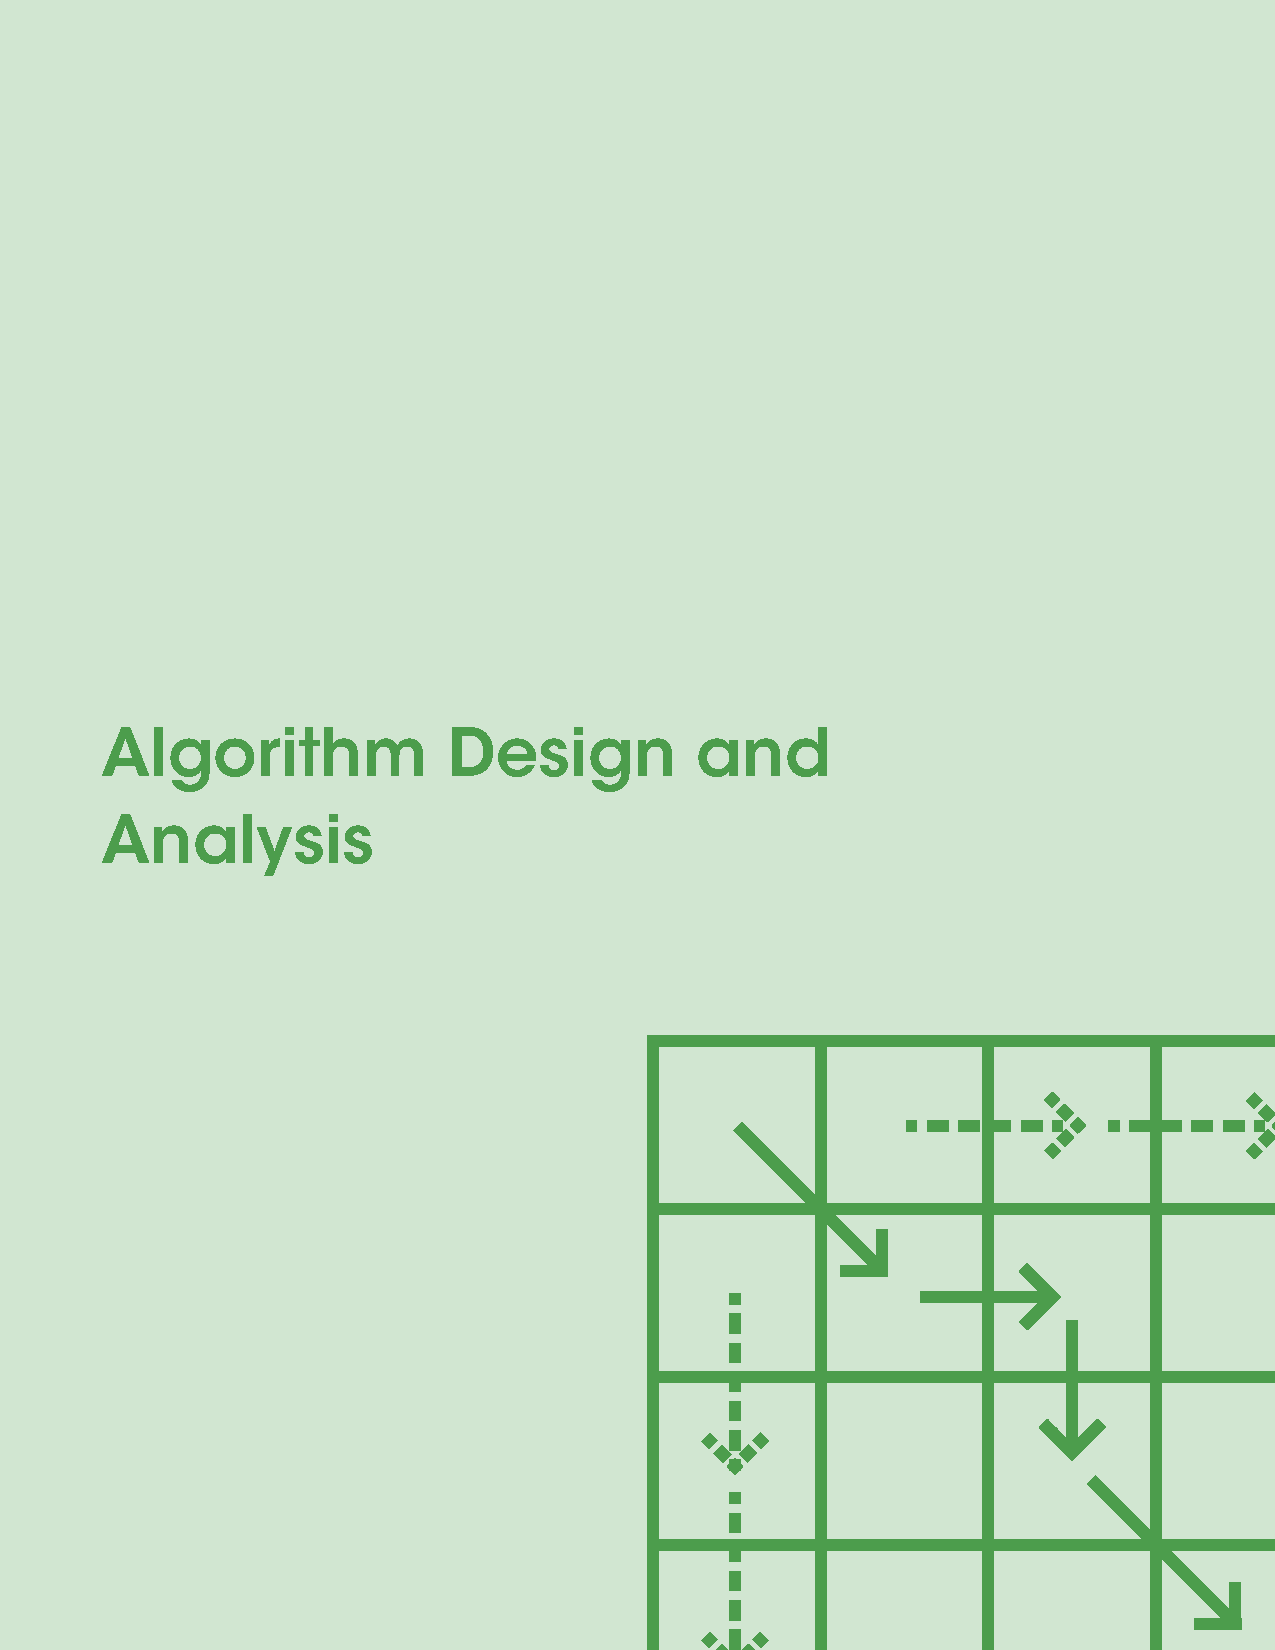
\includepdf[pages=-]{algo_cover.pdf}

%----------------------------------------------------------------------------------------
%	COPYRIGHT PAGE
%----------------------------------------------------------------------------------------

\newpage
The cover depicts a dynamic programming matrix used in the edit distance algorithm. Variations of this algorithm such as the Needleman-Wunsch and Smith-Waterman algorithms are frequently used in computational biology to align DNA or protein sequences.
~\vfill
\thispagestyle{empty}

\noindent Copyright \copyright\ \the\year{} Kevin Gao % Copyright notice

\hfill

\noindent \textsc{terra-incognita.dev} % URL

\hfill

% License information
\noindent Licensed under the Creative Commons Attribution-NonCommercial 3.0 Unported License (the ``License''). You may not use this file except in compliance with the License. You may obtain a copy of the License at \url{http://creativecommons.org/licenses/by-nc/3.0}. Unless required by applicable law or agreed to in writing, software distributed under the License is distributed on an \textsc{``as is'' basis, without warranties or conditions of any kind}, either express or implied. See the License for the specific language governing permissions and limitations under the License.


%----------------------------------------------------------------------------------------
%	TABLE OF CONTENTS
%----------------------------------------------------------------------------------------

%\usechapterimagefalse % If you don't want to include a chapter image, use this to toggle images off - it can be enabled later with \usechapterimagetrue

 % Table of contents heading image

\pagestyle{empty} % Disable headers and footers for the following pages
\usechapterimagefalse
\tableofcontents % Print the table of contents itself

\cleardoublepage % Forces the first chapter to start on an odd page so it's on the right side of the book

\pagestyle{fancy} % Enable headers and footers again

%----------------------------------------------------------------------------------------
%	PART
%----------------------------------------------------------------------------------------
\setlength{\parskip}{1em}

\part{Divide and Conquer}

\chapter{Divide and Conquer Primer}
\section{Divide and Conquer Paradigm}

Most divide and conquer algorithms follow this paradigm.

\begin{itemize}
    \item Divide up problem into several subproblems. Note that in some cases, we have to generalize the given problem.
    \item Recursively solving these subproblems.
    \item Combining the results from subproblems.
\end{itemize}

In this chapter and the following chapter, we will examine a few examples of divide-and-conquer algorithms, including but not limited to: maximum subarray, Strassen's matrix multiplication algorithm, quicksort, mergesort, median and selection in sorted array, fast Fourier transform (FTT), inversion counting, etc.

\section{The Master Theorem} \index{Master Theorem}

We have used the Master Theorem many times in both the introduction to theory of computation and data structure courses. We will once again present the theorem as it appears in CLRS here. For a careful proof of the theorem, see Section 4.6 of CLRS or Tutorial 7 note for CSC240 (Enriched Introduction to Theory of Computation).

\begin{theorem}[The Master Theorem]
    Let $a\geq 1$ and $b>1$ be constants, and let $f(n)$ be a function. Let $T(n)$ on the nonnegative integers by the recurrence
    $$
    T(n) = aT\left( \frac{n}{b} \right) + f(n)
    $$
    where $\frac{n}{b}$ is interchangeable with $\left\lfloor n/b \right\rfloor$ and $\left\lceil n/b \right\rceil $. Then, $T(n)$ has the following asymptotic bounds:
    \begin{itemize}
        \item If $f(n) \in O(n^{\log_b a - \epsilon})$ for some constant $\epsilon > 0$, then $T(n) \in \Theta(n^{\log_b a})$.
        \item If $f(n) \in \Theta(n^{\log_b a})$, then $T(n) \in \Theta(n^{\log_b a} \lg n)$.
        \item If $f(n) \in \Omega(n^{\log_b a+\epsilon})$ for some constant $\epsilon > 0$, and if $af(n/b) \leq cf(n)$ for some constant $c < 1$ and all sufficiently large $n$, then $T(n) \in \Theta(f(n))$. 
    \end{itemize}
\end{theorem}

An equivalent formulation of the theorem is as follows.

\begin{theorem}[The Master Theorem]
    Suppose that for $n \in \Z^+$.
    \begin{equation*}
        T(n) =
        \begin{cases}
        c & \text{if $n<B$} \\
        a_1 T(\lceil n/b \rceil) + a_2 T(\lfloor n/b \rfloor) + dn^i & \text{if $n\geq B$}
        \end{cases}
    \end{equation*}
    where $a_1, a_2, B, b \in \N$.
    
    Let $a = a_1+a_2 \geq 1$, $b>1$, and $c,d,i \in \R \cup \{0\}$. Then,
    \begin{equation*}
        T(n) \in
        \begin{cases}
        O(n^i \log n) & \text{if $a=b^i$} \\
        O(n^i) & \text{if $a < b^i$} \\
        O(n^{\log_b a}) & \text{if $a > b^i$}
        \end{cases}
    \end{equation*}
\end{theorem}

\section{Counting Inversions}

The objective of array inversion problems is to find the number inversions in an unsorted array compared to a sorted array. That is, given an array $A$, how many pairs $(i,j)$ are there such that $i < j$ and $A[i] > A[j]$. In other words, it counts the number of element-wise swaps needed in order to sort the given array.

For example, given the array $[8,4,2,1]$, the algorithm should answer 6 since the array has these six inversions: $(8,4)$, $(4,2)$, $(8,2)$, $(8,1)$, $(4,1)$, and $(2,1)$. If we follow these inversions, we will get a sorted array.

An naive algorithm for this problem is naturally to examine every pair of elements in the given array, which will take $O(n^2)$ comparisons. However, due to its resemblance to sorting, it is not hard to come up with a divide-and-conquer algorithm similar to mergesort that solves this problem in $O(n\log n)$ time.

At a high level, the algorithm should follow the aforementioned paradigm:
\begin{itemize}
    \item Divide: split list into two halves $A$ and $B$ 
    \item Conquer: recursively count inversions in each list
    \item Combine: count inversions $(a,b)$ with $a \in A$ and $b \in B$ 
    \item Return the sum of the tree counts
\end{itemize}

For the combine step, we assume that the two subarrays $A$ and $B$ are sorted. Then, we can scan $A$ and $B$ from left to right in parallel and compare $A[i]$ and $B[j]$. If $A[i] < B[j]$, then $A[i]$ is not inverted with any element in $B$. If $A[i] > B[j]$ then $B[j]$ is inverted with every element in left in $A$.

A pseudocode for the algorithm is shown below. Equivalently, instead of explicitly splitting the array, we can perform this in place by passing around the indices $p$ and $q$, as shown in Section 2.3.1 of CLRS.

\begin{codebox}
    \Procname{$\proc{Sort-And-Count}(L)$}
    \li \If $\attrib{L}{length} \isequal 0$ \Then
        \li \Return $(0,L)$ 
        \End
    \li $\id{mid} = \lfloor (1 + \attrib{L}{length})/2  \rfloor$
    \li $(\id{count-a}, A) = \proc{Sort-And-Count}(A[1\ldots \id{mid}])$
    \li $(\id{count-b}, B) = \proc{Sort-And-Count}(A[\id{mid}+1 \ldots \attrib{A}{length}])$ 
    \li $(\id{count-ab}, L') = \proc{Merge-And-Count}(A,B)$
    \li \Return $(\id{count-a}+\id{count-b}+\id{count-ab}, \, L')$ 
\end{codebox}

\begin{codebox}
    \Procname{$\proc{Merge-And-Count}(A,B)$}
    \li $\id{count} = 0$
    \li $i,j,k = 1$ 
    \li $L = []$ 
    \li \While $i \leq \attrib{A}{length}$ and $j \leq \attrib{B}{length}$ \Do
        \li \If $A[i] \leq B[j]$ \Then
            \li $L[k] = A[i]$
            \li $i = i + 1$
        \li \Else
            \li $\id{count} = \id{count} + 1$
            \li $L[k] = B[j]$
            \li $j = j + 1$
            \End
        \li $k = k + 1$
        \End
    \li \While $i \leq \attrib{A}{length}$ \Do
        \li $L[k] = A[i]$
        \li $k = k + 1$
        \End
    \li \While $j \leq \attrib{B}{length}$ \Do
        \li $L[k] = B[j]$
        \li $k = k + 1$
        \End
    \li \Return $(\id{count}, L)$ 
\end{codebox}

The number of comparisons made by the algorithm is given by this recurrence
$$
T(n) =
\begin{cases}
    \Theta(1) & \text{if $n = 1$} \\
    T(\lceil n/2 \rceil) + T(\lfloor n/2 \rfloor) + \Theta(n) & \text{otherwise}
\end{cases}
$$
By Masters Theorem, $T(n) \in O(n \log n)$.

\section{Closest Pair}

\vspace{\parskip}

\begin{lemma}
    Let $p$ be a point in the $2\delta$ strip within $\delta$ distance horizontally. There are at most 7 points $p$ such that $|y_p-y_q| \leq \delta$.
\end{lemma}

\begin{proof}
    $p$ must lie either in the left or right $\delta \times \delta$ square. Within each square, each point have distance at least $k$ from each other. So, we can pack at most 4 such points into one square, and since we have a left square and right square, we have 8 points in total. Other than $p$, there are at most 7 points.
\end{proof}

\begin{codebox}
    \Procname{$\proc{Closest-Pair}(P=p_1,p_2,\ldots,p_n)$}
    \li compute a vertical line $L$ such that half the points 
    \zi are on each side \RComment{$O(n \log n)$}
    \zi \Comment{consider sorting based on $x$-axis}
    \li $\delta_1 = \proc{Closest-Pair}(P_L)$
    \li $\delta_2 = \proc{Closest-Pair}(P_R)$
    \li $\delta = \min \{ \delta_1,\delta_2 \}$
    \li \For $p$ in $p_1,p_2,\ldots,p_n$ \Do \RComment{$O(n)$}
        \li \If $\proc{Y-Distance}(p,L)$ \Then
            \li \textbf{delete} $p$
        \End
    \End
    \li sort remaining points by $y$-coordinate \RComment{$O(n\log n)$}
    \li \For $p$ in $p_1,p_2,\ldots,p_n$ \Do \RComment{$O(n)$}
        \li \For $i$ \textbf{from} 1 \textbf{to} 7 \Do
            \li $p_i = \text{$i$th neighbor of $p$}$
            \li \If $\proc{Distance}(p,p_i) < \delta$ \Then
                \li $\delta = \proc{Distance}(p,p_i)$
            \End
        \End
    \End
    \li \Return $\delta$ 
\end{codebox}

The number of operations performed by this algorithm is
$$
T(n) =
\begin{cases}
    \Theta(1) & \text{if $n = 1$} \\
    T(\lceil n/2 \rceil) + T(\lfloor n/2 \rfloor) + O(n\log n) & \text{otherwise}
\end{cases}
$$
By Masters Theorem, $T(n) \in O(n \log^2 n)$.

\begin{theorem}[Lower Bound for Closest Pair]
    In a quadradic decision tree model, the closest pair problem requires at least $\Omega(n \log n)$ quadratic tests.
\end{theorem}

A quadradic decision tree is a comparison tree whose internal nodes are labeled with quadradic comparisons in the form of $x_i < x_j$ or $(x_i - x_k)^2 - (x_j - x_k)^2 < 0$. More generally, each internal node contains a comparison between a polynomial of degree at most 2 and 0 (2nd-order algebraic decision tree).

A hand-wavy proof of this lower bound follows by reduction from the result that the element uniqueness problem has a $\Omega(n \log n)$ lower bound, first shown by Ben-Or in \textit{Lower Bounds For Algebraic Computation Trees}. Element distinctness reduces to 2D closest pair problem.

\section{Karatsuba's Integer Multiplication Algorithm} \index{Karatsuba's algorithm}

To multiply two $n$-bit integers $a$ and $b$, we can follow this recursive procedure:
\begin{itemize}
    \item add two $\frac{1}{2}n$ bit integers
    \item multiply three $\frac{1}{2}n$-bit integers recursively
    \item add, subtract, and shift to obtain the result
\end{itemize}

$$
\begin{aligned}
    a &= 2^{n/2} a_1 + a_0 \\
    b &= 2^{n/2} b_1 + b_0 \\
    ab &= 2^n a_1b_1 + 2^{n/2} (a_1b_0 + a_0b_1) + a_0b_0 \\
    &= 2^n \underbrace{a_1b_1} + 2^{n/2} (\underbrace{(a_1+a_0)(b_1+b_0)} - \underbrace{a_1b_1} - \underbrace{a_0b_0}) + \underbrace{a_0b_0}
\end{aligned}
$$
The recursive steps are labeled with underbrace. By Masters Theorem, Karatsuba's algorithm performs
$$
T(n)=3T(\lceil n/2\rceil )+cn+d \in \Theta(n^{\log_2 3})
$$
bit-wise operations.

\chapter{Strassen's Algorithm}
\section{Matrix Multiplication}

The standard method to multiply two $n \times n$ matrices requires $O(n^3)$ scalar operations (multiplication and addition). The standard algorithm follows from the definition of matrix multiplication that the $i,j$ entry of $C=A \cdot B$ is given by
$$
c_{ij} = \sum_{k=1}^n a_{ik} \cdot b_{kj}
$$
\begin{codebox}
    \Procname{$\proc{Square-Matrix-Multiply}(A,B)$}
    \li $n = \attrib{A}{rows}$
    \li $C = \text{$n \times n$ matrix}$
    \li \For $i=1$ to $n$ \Do
        \li \For $j=1$ to $n$ \Do
            \li $c_{ij} = 0$
            \li \For $k=1$ to $n$ \Do
                \li $c_{ij} = c_{ij} + a_{ij}b_{ij}$
            \End
        \End
    \End
    \li \Return $C$ 
\end{codebox}
Clearly, this algorithm runs in $\Theta(n^3)$. 

\section{A Recursive Approach}

Without loss of generality, let $n=2^k$ for some $k$. Then, we can divide any $n \times n$ matrix into four $n/2 \times n/2$ matrices.
$$
\begin{bmatrix} C_{11} & C_{12} \\ C_{21} & C_{22} \end{bmatrix} = \begin{bmatrix} A_{11} & A_{12} \\ A_{21} & A_{22} \end{bmatrix}  \cdot \begin{bmatrix} B_{11} & B_{12} \\ B_{21} & B_{22} \end{bmatrix} 
$$
Since matrices are a non-commutative ring, $n \times n$ matrix multiplication can be realized in $7 n/2 \times n/2$ matrix multiplications and 18 matrix additions. Matrix addition only takes $O(n^2)$ scalar operations. Then, we have the following recurrence
$$
T(n) =
\begin{cases}
    1 & \text{if $n = 1$} \\
    7 T(n/2) + O(n^2) & \text{otherwise}
\end{cases}
$$
which implies that $T(n) \in O(n^{\log_2 7})$.

An implementation of this recursive approach is presented in pseudocode below
\begin{codebox}
    \Procname{$\proc{Square-Matrix-Multiply}(A,B)$}
    \li $n = \attrib{A}{rows}$
    \li $C = \text{$n\times n$ matrix}$ 
    \li \If $n \isequal 1$ \Then
        \li $c_{11} = a_{11} \cdot b_{11}$
    \Else
        \li partition $A$, $B$, and $C$ each into four sub-matrices
        \li $C_{11} = \proc{Square-Matrix-Multiply}(A_{11},B_{11}) + $
        \zi \> $\phantom{=}\proc{Square-Matrix-Multiply}(A_{12},B_{21})$
        \li $C_{12} = \proc{Square-Matrix-Multiply}(A_{11},B_{12}) + $
        \zi \> $\phantom{=}\proc{Square-Matrix-Multiply}(A_{12},B_{22})$
        \li $C_{21} = \proc{Square-Matrix-Multiply}(A_{21},B_{11}) + $
        \zi \> $\phantom{=}\proc{Square-Matrix-Multiply}(A_{22},B_{21})$
        \li $C_{22} = \proc{Square-Matrix-Multiply}(A_{21},B_{12}) + $
        \zi \> $\phantom{=}\proc{Square-Matrix-Multiply}(A_{22},B_{22})$
    \End
    \li \Return $C$ 
\end{codebox}
However, this particular implementation of the recursive approach still has a $O(n^3)$ running time, as demonstrated by solving the recurrence by Masters Theorem.

\section{Strassen's Algorithm}

Strassen's algorithm is a rather peculiar algorithm that multiplies two square matrices using $O(n^{\log_2 7}) = O(n^{2.81})$ scalar operations. It is debatable how practical asymptotically faster matrix multiplication algorithms (including Strassen's algorithm and Coppersmith-Winograd algorithm) are given that their crossover point (the threshold on input size beyond which such algorithms become actually faster) is often quite large for them to be useful in practical applications.

Strassen's algorithm as described in CLRS works as follows:
\begin{enumerate}
    \item Divide the input matrices $A$ and $B$ and output matrix $C$ into $n/2 \times n/2$ submatrices. This takes $\Theta(1)$ operations.
    \item Create 10 submatrices $S_1,S_2,\ldots,S_{10}$, each of which is $n/2 \times n/2$ and is the sum or difference of two matrices created in Step 1. This can be done in $\Theta(n^2)$.
    \item Using the submatrices in Step 1 and the 10 matrices in Step 2, recursively compute seven matrix products $P_1,P_2,\ldots,P_7$. Each matrix $P_i$ is $n/2 \times n/2$.
    \item Compute the desired $C_{11},C_{12},C_{21},C_{22}$ of the result matrix $C$ by adding and subtracting various combinations of the $P_i$ matrices. This can also be done in $\Theta(n^2)$ time.
\end{enumerate}
More specifically, in Step 2,
$$
\begin{aligned}
    S_1 &= B_{12} - B_{22} \\
    S_2 &= A_{11} + A_{12} \\
    S_3 &= A_{21} + A_{22} \\
    S_4 &= B_{21} - B_{11} \\
    S_5 &= A_{11} + A_{22} \\
    S_6 &= B_{11} + B_{22} \\
    S_7 &= A_{12} - A_{22} \\
    S_8 &= B_{21} + B_{22} \\
    S_9 &= A_{11} - B_{21} \\
    S_{10} &= B_{11} + B_{12},
\end{aligned}
$$
and in Step 3,
$$
\begin{aligned}
    P_1 &= A_{11} \cdot S_1 &=& A_{11} \cdot B_{12} - A_{11} \cdot B_{22} \\
    P_2 &= S_2 \cdot B_{22} &=& A_{11} \cdot B_{22} + A_{12} \cdot B_{22} \\
    P_3 &= S_3 \cdot B_{11} &=& A_{21} \cdot B_{11} + A_{22} \cdot B_{11} \\
    P_4 &= A_{22} \cdot S_4 &=& A_{22} \cdot B_{21} - A_{22} \cdot B_{11} \\
    P_5 &= S_5 \cdot S_6 &=& A_{11} \cdot B_{11} + A_{11} \cdot B_{22} + A_{22} \cdot B_{11} + A_{22} \cdot B_{22} \\
    P_6 &= S_7 \cdot S_8 &=& A_{12} \cdot B_{21} + A_{12} \cdot B_{22} - A_{22} \cdot B_{21} - A_{22} \cdot B_{22} \\
    P_7 &= S_9 \cdot S_{10} &=& A_{11} \cdot B_{11} + A_{11} \cdot B_{12} - A_{21} \cdot B_{11} - A_{21} \cdot B_{12}.
\end{aligned}
$$
In Step 4,
$$
\begin{aligned}
    C_{11} &= P_5 + P_4 - P_2 + P_6 \\
    C_{12} &= P_1 + P_2 \\
    C_{21} &= P_3 + P_4 \\
    C_{22} &= P_5 + P_1 - P_3 - P_7
\end{aligned}
$$

\chapter{Fast Fourier Transform}
\section{Motivation}
A polynomial can be represented in various ways. Each representation has its advantages and downsides.

In general, a polynomial $A(x)$ of degree $n-1$ can be written as
$$
\begin{aligned}
    A(x) &= a_0 + a_1x + a_2x^2 + \cdots + a_{n-1}x^{n-1} \\
    &= \sum_{k=0}^{n-1} a_k x^k
\end{aligned}
$$

\subsection{Coefficient Vector}

For a polynomial $A(x)$ of degree $n-1$, the coefficient vector contains the coefficient of the polynomial represented as a vector.
$$
A(x) = a_0 + a_1 x + a_2 x^2 + \cdots + a_{n-1}x^{n-1} \quad  \leftrightarrow \quad \langle a_0,a_1,a_2,\ldots,a_{n-1} \rangle
$$

\subsection{Roots}

Equivalently,
$$
A(x) = (x-r_0) (x-r_1) \cdots (x - r_{n-1}) \cdot c
$$
where $r_0,r_1,\ldots,r_{n-1}$ are the $n$ roots of the polynomial and $c$ is a scale term.

\subsection{Samples}

Given a polynomial, we can take $n$ points (coordinates): 
$$
(x_0,y_0),\, (x_1,y_1),\, \ldots ,\, (x_{n-1},y_{n-1})
$$
where $A(x_i)=y_i$ for all $i \in \{0,1,\ldots,n-1\}$. This representation is also known as the point-value representation.

By the Foundamental Theorem of Algebra, these samples uniquely define a polynomial of degree $n-1$.

\begin{theorem}[The Fundamental Theorem of Algebra]
    A univariate polynomial of degree $n$ with complex coefficients has exactly $n$ complex roots.
\end{theorem}

\begin{corollary}[Uniqueness of Polynomial Interpolation]
    A degree $n-1$ univariate polynomial $A(x)$ is uniquely defined by its evaluation at $n$ distinct values of $x$.
\end{corollary}

\section{Operations on Polynomials}

There are three primary operations on polynomials: evaluation, addition, and multiplication. The complexity of these operations varies depending on the representation. There is not a single representation that is efficient for all operations, so we need a way to efficiently convert between the representations. 

\subsection{Coefficient Representation}

\subsubsection{Evaluation}

Evaluation is efficient when the polynomial is represented as the coefficient vector using the Horner's rule:
$$
A(x_0) = a_0 + x_0 (a_0 + x_0 (a_2 + \cdots + x_0 (a_{n-2} + x_0 (a_{n-1})) \cdots ))
$$
which can be written in pseudocode as follows
\begin{codebox}
    \Procname{$\proc{Evaluate}(A=\langle a_0,\ldots a_{n-1}\rangle,\,x)$}
    \li $y = 0$
    \li \For $i = n-1$ \textbf{to} 0 \Do
        \li $y = a_j + (x \cdot y)$
    \End
    \li \Return $y$ 
\end{codebox}

\subsubsection{Addition}

Addition is easy in coefficient representation. We simply add each coefficient to get a new coefficient vector.

\begin{codebox}
    \Procname{$\proc{Add}(A=\langle a_0\ldots a_{n-1} \rangle,\, B=\langle b_0 \ldots b_{n-1} \rangle)$}
    \li \For $j = 0$ \textbf{to} $n-1$ \Do
        \li $c_j = a_j + b_j$
    \End
    \li \Return $C = \langle c_0,\ldots,c_{n-1} \rangle$
\end{codebox}

\subsubsection{Multiplication}

Multiplication is a little bit trickier in coefficient representation. We need to use linear convolution, which takes $O(n^2)$ operations.
$$
A(x) \times B(x) = \sum_{j=0}^{2n-2} c_j x^j = \sum_{j=0}^{2n-2} \sum_{k=0}^j a_k b_{j-k} x^j
$$
\begin{codebox}
    \Procname{$\proc{Multiply}(A=\langle a_0\ldots a_{n} \rangle,\, B=\langle b_0 \ldots b_{m} \rangle)$}
    \li \For $j = 0$ to $n+m$ \Do
        \li $c_j = 0$
    \End
    \li \For $j = 0$ to $n$ \Do
        \li \For $k = 0$ to $n$ \Do
            \li $c_{j+k} = c_{j+k} + a_j \cdot b_k$
        \End
    \End
    \li $C = \langle c_0 \ldots c_{n+m} \rangle$
\end{codebox}

\subsection{Samples}

\subsubsection{Evaluation}

Evaluation can be done in $O(n^2)$ through interpolation using Lagrange's formula.
$$
A(x) = \sum_{k=0}^{n-1} y_k \frac{\prod_{j\neq k} (x-x_j)}{\prod_{j \neq k} (x_k - x_j)}
$$

\subsubsection{Addition}

Addition is also easy in samples representation.
$$
A(x) + B(x):\; (x_0,y_0+z_0),(x_1,y_1+z_1),\ldots (x_{n-1},y_{n-1}+z_{n-1})
$$
given that $A(x)$ is represented as $(x_0,y_0),\ldots,(x_{n-1},y_{n-1})$ and \\ $B(x)$ is represented as $(x_0,z_0),\ldots,(x_{n-1},z_{n-1})$.

\subsubsection{Multiplication}

Multiplication is done in a similar fashion as addition.
$$
A(x) \times B(x):\; (x_0,y_0z_0),(x_1,y_1z_1),\ldots (x_{n-1},y_{n-1}z_{n-1})
$$
given that $A(x)$ is represented as $(x_0,y_0),\ldots,(x_{n-1},y_{n-1})$ and \\ $B(x)$ is represented as $(x_0,z_0),\ldots,(x_{n-1},z_{n-1})$.

\subsection{Roots}
\subsubsection{Evaluation}
Takes $O(n)$ operations by substitution and multiplication.

\subsubsection{Addition}
Impossible in the general case. There is not a general formula that can converts a coefficient vector back to the roots.

\subsubsection{Multiplication}
Multiplying two polynomials represented by their roots is equivalent to concatenate the list of roots since the resulting polynomial will have the the same roots of both polynomials.

\subsection{Summary}

\begin{table}[htpb]
    \centering
    \begin{tabular}{c|c|c|c}
    & Coefficient & Roots & Samples \\
    \hline
    Evaluation & $O(n)$ & $O(n)$ & $O(n^2)$ \\
    \hline
    Addition & $O(n)$ & $\infty$ & $O(n)$ \\
    \hline
    Multiplication & $O(n^2)$ & $O(n)$ & $O(n)$  
    \end{tabular}
    \caption{Comparison between different representations of polynomial}
    \label{tab:polynomial-rep-comparison}
\end{table}

The following chart outlines the conversions required for efficient multiplication of polynomials. The figure is taken from CLRS pp. 904.

\begin{figure}[htbp]
    \centering
    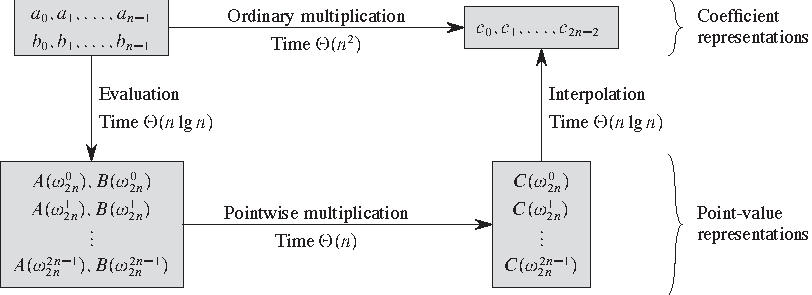
\includegraphics{fft/polynomial-conversion.pdf}
    \caption{Graphical outline of an efficient polynomial multiplication procedure.}
    \label{fig:fft-polynomial-conversion}
\end{figure}

\section{Fast Fourier Transform}

\subsection{Coefficient to Samples (and back)}

Conversion from coefficient to samples is similar to evaluation. We fix a set of points $x_0,x_1,\ldots,x_{n-1}$ and evaluate the polynomial at these points. This evaluation is equivalent to the following matrix multiplication
$$
\mathbf{y} = \mathbf{V} \mathbf{a} =
\begin{bmatrix}
1 & x_0 & x_0^2 & \cdots & x_0^{n-1} \\
1 & x_1 & x_1^2 & \cdots & x_1^{n-1} \\
1 & x_2 & x_2^2 & \cdots & x_2^{n-1} \\
\vdots & \vdots & \vdots & \ddots & \vdots \\
1 & x_{n-1} & x_{n-1}^2 & \cdots & x_{n-1}^{n-1} \\
\end{bmatrix}
\begin{bmatrix} 
    a_0 \\
    a_1 \\
    a_2 \\
    \vdots \\
    a_{n-1}
\end{bmatrix} =
\begin{bmatrix} 
    y_0 \\
    y_1 \\
    y_2 \\
    \vdots \\
    y_{n-1}
\end{bmatrix} 
$$
where $\mathbf{V}$ is called the Vandermonde matrix with entries $V_{jk} = x_j^k$ and $\mathbf{a}$ is the coefficient vector of the polynomial $A(x)$.

Evaluating this matrix product takes $\Theta(n^2)$ scalar operations. Similarly, to convert from samples back to polynomial (interpolation), we can compute $\mathbf{V}^{-1}$ using Gaussian elimination with $O(n^3)$ operations, and computing $\mathbf{a} = \mathbf{V}^{-1}\mathbf{y}$ (it is rarely a good idea to invert any matrices; ``Don't invert that matrix!'' -- John Cook).

In order to obtain efficient algorithms for manipulating polynomials, we need to somehow get rid of the $O(n^2)$ overhead resulted from the interconversion between coefficient and samples.

Note that we simply said ``fix $x_0\ldots x_{n-1}$'' when constructing the Vandermonde matrix without putting any constraints on what values of $x$ to take. By choosing special values for $x$, we can reduce the conversion overhead to $O(n \log n)$.

\subsection{Divide and Conquer}

We can formulate the evaluation $\mathbf{y}=\mathbf{V}\mathbf{a}$ as a divide and conquer algorithm.

We can come up with an outline of the algorithm by following the divide-and-conquer paradigm
\begin{enumerate}
    \item Divide: divide the polynomial $A$ into even and odd coefficients (this is equivalent to divide the coefficient vector $\mathbf{a}$ into even and odd entries)
    $$
    A_{even}(x) = \sum_{k=0}^{\lceil \frac{n}{2}-1 \rceil} a_{2k}x^k \quad \leftrightarrow \quad \mathbf{a}_{even} = \langle a_0,a_2,a_4,\ldots \rangle
    $$
    $$
    A_{odd}(x) = \sum_{k=0}^{\lfloor \frac{n}{2}-1 \rfloor} a_{2k+1}x^k \quad \leftrightarrow \quad \mathbf{a}_{odd} = \langle a_0,a_2,a_4,\ldots \rangle
    $$
    Note that the degree of the two resulting polynomials is half of the original polynomial.

    \item Conquer: recursive conquer $A_{even}(x)$ and $A_{odd}(x)$ for $x \in X^2$ where $X^2 = \{x^2 \mid x \in X\}$.
    
    \item Combine: combine the terms as follows
    $$
    A(x) = A_{even}(x^2) + xA_{odd}(x^2)
    $$
    for $x \in \mathbf{x}$.
\end{enumerate}

It is obvious that the degree of the polynomial $n$ halves, and hence the recurrence
$$
T(n,|X|) = 2T\left( \frac{n}{2},|X| \right) + O(n + |X|) \in O(n^2).
$$
This is no better than the naive approach. The main issue is that we are not halving the size of $X$. Ideally, we want $X$ to be recursively collapsing.

\subsection{Complex Roots of Unity} \index{complex roots of unity}

We can construct a collapsing set of $x$'s via square roots. If we only look at real numbers, taking the square root or squaring a number won't give you fewer or more numbers, but if we broaden our view to complex numbers, we notice that starting from 1, every time we take the square root, the size of the set doubles. The $n$th root of 1 is called the \textit{\textbf{complex $n$th root of unity}}. The observation implies that if we start from the $n$th root of unity and square the elements in the set, the set will collapse every time we square it.

Example: $\{1\} \to \{1,-1\} \to \{1,-1,i,-i\} \to \{1,-1,i,-i,\pm \frac{\sqrt{2}}{2}(1+i),\pm \frac{\sqrt{2}}{2}(-1+i) \}$

The complex roots of unity are spaced equally around the unit circle centered at the origin of the complex plane. These points are of the form $\cos\theta + i\sin\theta = e^{i\theta}$ for $\theta = 0,\frac{2}{n}\pi,\frac{4}{n}\pi,\ldots,\frac{2(n-1)}{n}\pi$. 

\begin{center}
    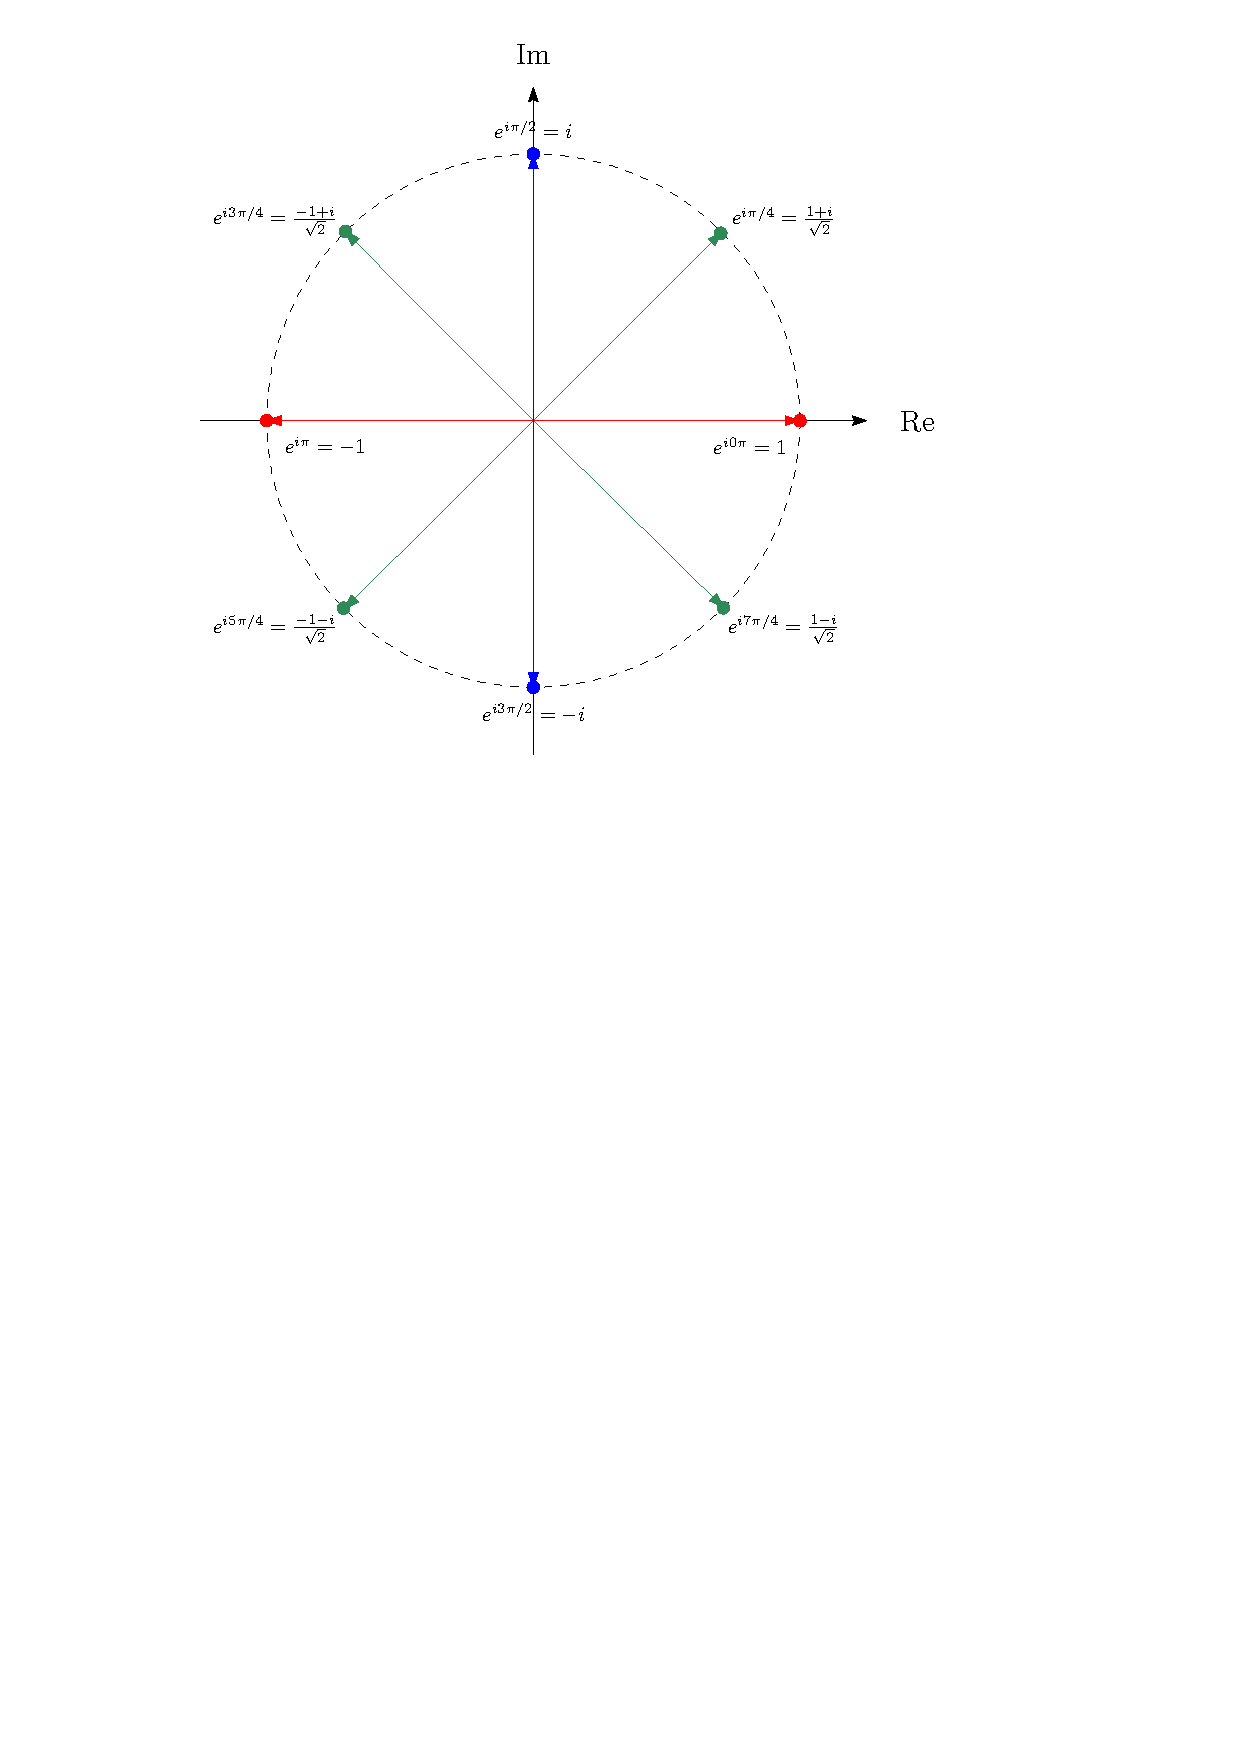
\includegraphics[width=0.6\linewidth]{fft/nth-root-of-unity.pdf}
\end{center}

The $n$th roots of unity where $n=2^\ell$ for some integer $\ell$ form a collapsing set since $(e^{i\theta})^2 = e^{i 2\theta} = e^{i(2\theta \bmod 2\pi)}$. 

Let us formalize this idea and prove that it works.

\begin{lemma}[Halving (Collapsing) Lemma]
    If $n>0$ is even, then the squares of the $n$ complex $n$th roots of unity are the $n/2$ complex $(n/2)$th roots of unity. 
\end{lemma}

\begin{proof}
    We know that $\left(e^{\frac{2\pi i}{n}}\right)^{2k} = e^{\frac{4k\pi i}{n}} = \left(e^{\frac{2\pi i}{1/2 \cdot n}}\right)^k$ for any nonnegative integer $k$. 
    
    Furthermore, $\left(e^{\frac{2\pi i}{n}}\right)^{2(k+n/2)} = \left(e^{\frac{2\pi i}{n}}\right)^{k}$. This implies that for every pair of $k$ and $k+n/2$ share the same square, and that if take the square of every element in the set of $n$th roots of unity, we get the $n/2$ elements and it follows from algebra that the resulting set contains the $(n/2)$th roots of unity.
\end{proof}

\subsection{The FFT Algorithm} \index{fast Fourier transform (FFT)}

By choosing the $x$'s in the Vandermonde matrix to be the $n$th roots of unity, we can make $X$ collapsing along with $n$. The rest of the algorithm is the same as the divide-and-conquer approach described earlier.

\begin{codebox}
    \Procname{$\proc{FFT-Recursive}(a)$}
    \li $n = \attrib{a}{length}$
    \li \If $n \isequal 1$ \Then
        \li \Return $a$ 
    \End
    \li $\omega_n = e^{2\pi i/n}$
    \li $\omega = 1$
    \li $a_{even} = (a_0,a_2,\ldots,a_{n-2})$
    \li $a_{odd} = (a_1,a_3,\ldots,a_{n-1})$
    \li $y_{even} = \proc{FFT-Recursive}(a_{even})$
    \li $y_{odd} = \proc{FFT-Recursive}(a_{odd})$
    \li \For $k = 0$ to $n/2 - 1$ \Do
        \li $y_k = y_{even}[k] + \omega y_{odd}[k]$
        \li $y_{k+\frac{n}{2}} = y_{even}[k] - \omega y_{odd}[k]$
        \li $\omega = \omega \omega_n$
    \End
    \li \Return $y = (y_0,\ldots,y_{n-1})$      
\end{codebox}

This algorithm takes $T(n) = 2T\left( \frac{n}{2} \right) + O(n) \in O(n \log n)$ operations.

\section{Inverse Fast Fourier Transform} \index{inverse fast Fourier transform (IFFT)}

The inverse discrete fourier transform is an algorithm used to find the coefficients fo a polynomial given a set of samples. The transformation is of the form $\mathbf{a}^* \to \mathbf{V}^{-1}\mathbf{a}^* = \mathbf{a}$. To evaluate this, we need $\mathbf{V}^{-1}$. In fact, this matrix has a very useful property that allows to find it without actually inverting $\mathbf{V}$ (again, don't invert the matrix).

\begin{lemma}
    Let $\mathbf{V}$ be the Vandermonde matrix constructed from the set of $n$th roots of unity. Let $\overline{\mathbf{V}}$ denote the complex conjugate of $\mathbf{V}$. Then,
    $$
    \mathbf{V}^{-1} = \frac{1}{n}\overline{\mathbf{V}}
    $$
\end{lemma}

\begin{proof}
    We claim that $\mathbf{P} = \mathbf{V}\overline{\mathbf{V}} = n \mathbf{I}$.

    Let $p_{jk}$ be the $j,k$th entry of $\mathbf{P}$.
    $$
    \begin{aligned}
        p_{jk} &= (\text{row $j$ of $\mathbf{V}$}) \cdot (\text{column $k$ of $\overline{\mathbf{V}}$}) \\
        &= \sum_{m=0}^{n-1} e^{ij2\pi m/n} \overline{e^{ik2\pi m/n}} \\
        &= \sum_{m=0}^{n-1} e^{ij2\pi m/n} e^{-ik2\pi m/n} \\
        &= \sum_{m=0}^{n-1} e^{i(j-k)2\pi m/n}
    \end{aligned}
    $$
    Take $j=k$. Then, $p_{jk} = \sum_{m=0}^{n-1} 1 = n$. Otherwise, $p_{jk} = 0$. This means that the diagonal entries are $n$, and the entires off the diagonal are all 0. Thus, the claim is true.

    It follows that $\mathbf{V}^{-1} = 1/n \mathbf{V}$.
\end{proof}

This lemma implies that for the Inverse Fast Fourier Transform algorithm, we can simply replace $e^{ikr/n}$ with its complex conjugate in the FFT algorithm and divide the final result by 2. The rest of the algorithm is analogous to that for FFT, and it is easy to see that the running of IFFT is also in $O(n \log n)$.

Quite surprisingly, many sources online including lecture notes from numerous institutions and prominant YouTube channels appear to have made some mistakes when presenting the pseudocode for IFFT. For a recursive implementation, the division by $n$ is applied only once at the very end when all recursive calls have terminated, not during the recursive call. It is not correct to simply change the twiddle factor to $w_n = e^{-2\pi i/n} / n$ or to divide by $n$ every time we update $a$ like $a_k = (a_{even}[k] + \omega a_{odd}[k])\; / n$. However, it is correct to divide by 2 every time we update $a$, as shown below. It is the same implementation as the one in Jeff Erickson's notes.

\begin{codebox}
    \Procname{$\proc{IFFT-Recursive}(y)$}
    \li $n = \attrib{y}{length}$
    \li \If $n \isequal 1$ \Then
        \li \Return $y$ 
    \End
    \li $\omega_n = e^{{\color{red}-}2\pi i/n}$
    \li $\omega = 1$
    \li $y_{even} = (y_0,y_2,\ldots,y_{n-2})$
    \li $y_{odd} = (y_1,y_3,\ldots,y_{n-1})$
    \li $a_{even} = \proc{IFFT-Recursive}(y_{even})$
    \li $a_{odd} = \proc{IFFT-Recursive}(y_{odd})$
    \li \For $k = 0$ to $n/2 - 1$ \Do
        \li $a_k = (a_{even}[k] + \omega a_{odd}[k])\; {\color{red} / \;2}$
        \li $a_{k+\frac{n}{2}} = (a_{even}[k] - \omega a_{odd}[k])\; {\color{red} / \;2}$
        \li $\omega = \omega \omega_n$
    \End
    \li \Return $a = (a_0,\ldots,a_{n-1})$      
\end{codebox}

\section{Fast Polynomial Multiplication}

With FFT, we can implement the procedure outlined in Figure \ref{fig:fft-polynomial-conversion}.

To calculate $A(x)\times B(x)$,

\begin{enumerate}
    \item Compute $A^* = \proc{FFT}(A)$ and $B^* = \proc{FFT}(B)$. This step is $O(n \log n)$.
    \item Compute $C^* = A^* \cdot B^*$ in sample representation. This step is $O(n)$.
    \item Compute $C = \proc{IFFT}(C^*)$ to get $C$ in coefficient representation. This step is $O(n \log n)$.
\end{enumerate}
Overall, the algorithm has runtime complexity of $O(n \log n)$.

\part{Greedy Algorithms}

\chapter{Interval Scheduling}
\section{Interval Scheduling}

We begin by considering the interval scheduling problem. The same problem is referred to as the activity selection problem in CLRS.

Consider a set $S = \{a_1,a_2,\ldots,a_n\}$ of jobs/activities, each with a start time $s_i$ and finish time $f_i$. Two jobs are said to be compatible if they don't overlap. More formally, given activities $a_i$ and $a_j$, they are compatible if $[s_i,f_i) \cap [s_j,f_j) = \emptyset$. That is, if $s_i \geq f_j$ or $s_j \geq f_i$. The goal of the interval scheduling problem is to find a maximum-size subset of mutually compatible jobs.

Let us consider the greedy strategy for solving the interval scheduling problem. Intuitive, the globally optimal solution should leave resources/time open for as many other jobs as possible. This requires us to consider the jobs in some ``natural'' order:

\begin{itemize}
    \item Earliest start time: consider jobs in ascending order of $s_i$
    \item Earliest finish time: consider jobs in ascending order of $f_i$
    \item Shortest inverval: consider jobs in ascending order of $f_i - s_i$ 
    \item Fewest conflicts: for each job $a_i$, count the remaining number of conflicting jobs $c_i$ and schedule in ascending order of $c_i$. 
\end{itemize}

Not all of those strategies work. Here are some counterexamples (Figure \ref{fig:greedy-interval-scheduling-counterexample}).

\begin{figure}[htbp]
    \centering
    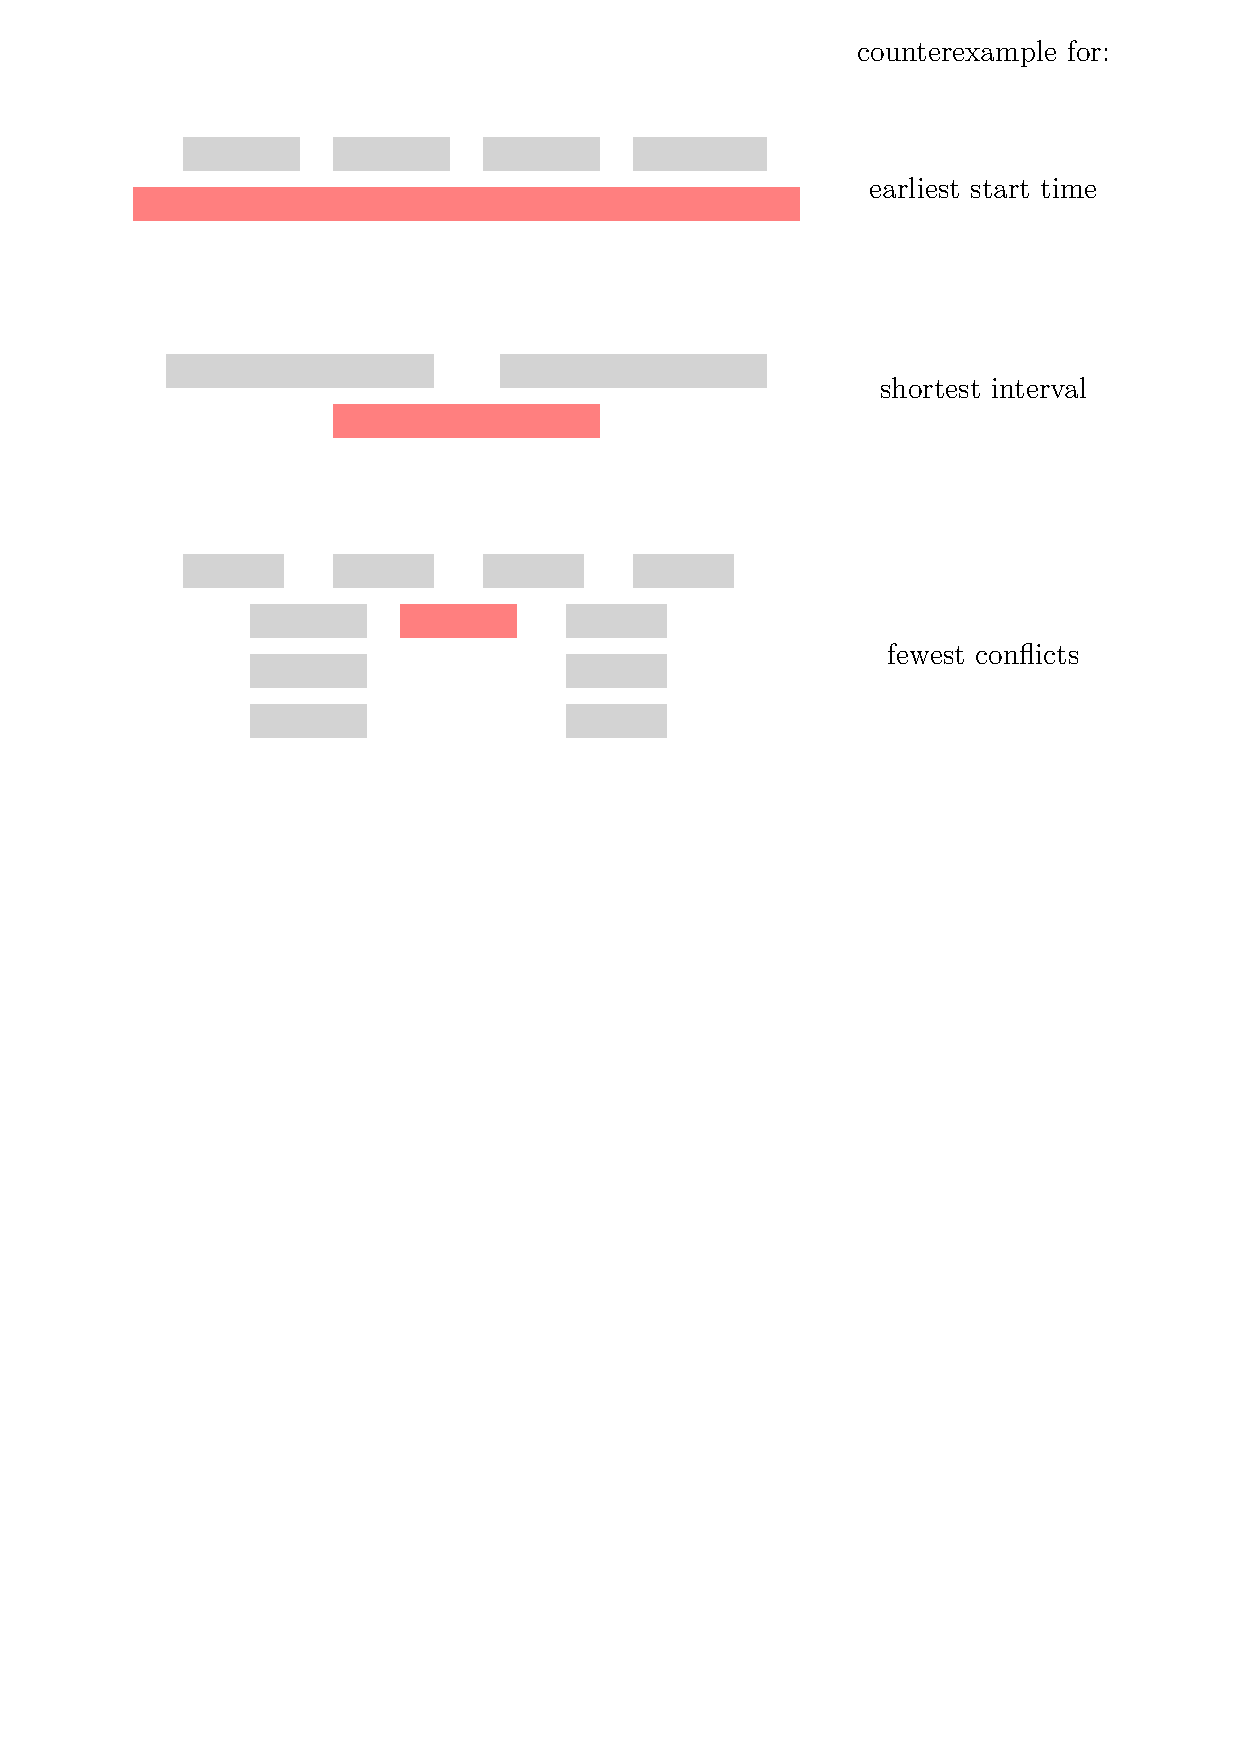
\includegraphics[width=0.7\linewidth]{greedy/interval-scheduling-counterexample.pdf}

    \hfill

    \caption{Counterexamples for the greedy strategies that do not work for the interval scheduling problem. The interval that satisfies the greedy strategy but leads to incorrect global solution is highlighted in red.}
    \label{fig:greedy-interval-scheduling-counterexample}
\end{figure}

Therefore, we choose earliest finish time as our greedy strategy, which we can implement into this recursive algorithm

\begin{codebox}
    \Procname{$\proc{Interval-Scheduling-Recursive}(S,k,n)$}
    \li $m = k + 1$
    \li \While $m \leq n$ and $S[m].s < S[k].f$ \Do
        \li $m = m + 1$
    \End
    \li \If $m \leq n$ \Then
        \li \Return $\{S[m]\} \cup \proc{Interval-Scheduling-Recursive}(S,m,n)$
    \li \Else
        \li \Return $\emptyset$ 
\end{codebox}

As a precondition, we assume that the array of jobs $S$ is sorted in monotonically increasing order by finish time. $S[i].s$ denotes the starting time of the $i$th job, and $S[i].f$ denotes the finish time of the $i$th job. $k$ is the job being considered. In each call to the recursive algorithm, we starts from $m = k+1$ and increment $m$ until we find a job with starting time $S[m].s$ strictly lower than the finish time of $S[k]$. This is the job that is selected by our greedy strategy in the current recursive call. After finding this $m$, we return the union of $\{S[m] = a_m\}$ and the maximum-size subset of $S_m$ returned by the recursive call $\proc{Interval-Scheduling-Recursive}(S,m,n)$.

The initial call that solves the problem globally is $\proc{Interval-Scheduling-Recursive}(S,0,n)$ where $n$ is the number of jobs to be considered.

This algorithm can be easily converted into an iterative algorithm.

\begin{codebox}
    \Procname{$\proc{Interval-Scheduling}(S)$}
    \li $n = \attrib{S}{length}$ 
    \li $S' = \{a_1\}$
    \li $k = 1$
    \li \For $m = 2$ to $n$ \Do
        \li \If $S[m].s \geq S[k].f$ \Then
            \li $S' = S' \cup \{S[m]\}$
            \li $k = m$
        \End
    \End
    \li \Return $S'$ 
\end{codebox}

Sorting the array of jobs takes $O(n \log n)$ time, and going over the sorted the list and check each job's compatibility takes $O(n)$ in total.

\section{Proving Optimality}

As we have demonstrated earlier in Figure \ref{fig:greedy-interval-scheduling-counterexample}, greedy strategy does not always work. It is important for us to ensure (prove) that the locally optimal greedy choice leads to a globally optimal solution. Here, we will present three equally valid proofs for the optimality of the greedy algorithm for the interval scheduling problem.

\begin{theorem}
    The greedy algorithm using earliest finish time is optimal. More formally, the algorithm returns a maximum-size set of disjoint jobs $\{a_1,\ldots,a_m\} \subseteq S$
\end{theorem}

\begin{proof}[Proof (by contradiction)]
    Suppose, for contradiction, that the greedy algorithm using earlies finish time is not optimal. Let $i_1,i_2,\ldots,i_k$ be the sequence of jobs selected by the algorithm, and let $j_1,j_2,\ldots,j_m$ be the correct solution where $m>k$. Let $r$ be the largest possible value such that $i_{r+1} \neq j_{r+1}$. That is, the $(r+1)$th job is the first job where the two sequences begin to differ. 

    Both $i_{r+1}$ and $j_{r+1}$ must be compatible with previous choices of $i$ and $j$, respectively. Let $i_1=j_1,i_2=j_2,\ldots,i_r=j_r,i_{r+1},j_{r+2}, \ldots, j_m$ be a new sequence of jobs. This is the optimal solution with $j_{r+1}$ replaced with $i_{r+1}$. By assumption, the greedy solution is not optimal so $j_{r+1}$ is not selected by the greedy algorithm and thus $i_{r+1} \leq j_{r+1}$. So, the new sequence of jobs is still feasible because $i_{r+1} \leq j_{r+1}$. The algorithm is still optimal because all $m$ disjoint jobs are scheduled. But then, $i_{r+1}$ is not different from $j_{r+1}$, which implies that $r$ is not the maximum value such that $i_{r+1} \neq j_{r+1}$. This is a contradiction. Therefore, the greedy algorithm is optimal.
\end{proof}

\begin{proof}[Proof (by induction)]
    Let $S_k$ be the subset of jobs selected by the greedy algorithm after considering the first $k$ jobs in increasing order of finish time. We say that $S_k \subseteq S$ is promising if it can be extended to the optimal solution ($S_k$ is part of the optimal solution). More formally, $S_k$ is promising if there exists $T \subseteq \{ a_{k+1},\, \ldots,\, a_{n}\}$ such that $O_k = S_k \cup T$ is optimal.

    We want to show that for all $k \in \{0,1,\ldots,n\}$, $S_k$ is promising.

    \textbf{Base case}: When $k=0$, $S_0=\emptyset$. The claim is vacuously true.
    
    \textbf{Inductive step}: Let $j \in \N$ be arbitrary. Suppose that the claim holds for $k = j - 1$ and that $S_{j-1}$ is promising. For $S_j$, there are two possibilities:

    (1) The greedy algorithm did not select job $a_j$ (i.e. $s_{j+1} < f_j$), so $S_j = S_{j-1}$. This implies that $a_j$ is not compatible with some job in $S_{j-1}$. Since $S_{j-1} \subseteq O_{j-1}$, $O_{j-1}$ does not include $a_j$. $O_j = O_{j-1}$ does not include $a_j$, so $S_j$ can be extended to $O_j$ and $S_j$ is promising.
    
    (2) The greedy algorithm selected job $a_j$ (i.e. $s_{j+1} \geq f_j$), so $S_j = S_{j-1} \cup \{a_j\}$. Consider the earliest job $a_r$ in $O_{j-1} - S_{j-1}$. Consider $O_j = O_{j-1} - \{a_r\} \cup \{a_j\}$. $O_j$ is still feasible since jobs in $O_{j-1}$ are disjoint, $a_r$ is the first to finish, and the finish time of $a_j$ is earlier or equal to the finish time of $a_r$. Hence, $S_j$ can be extended to $O_j$.

    \begin{center}
        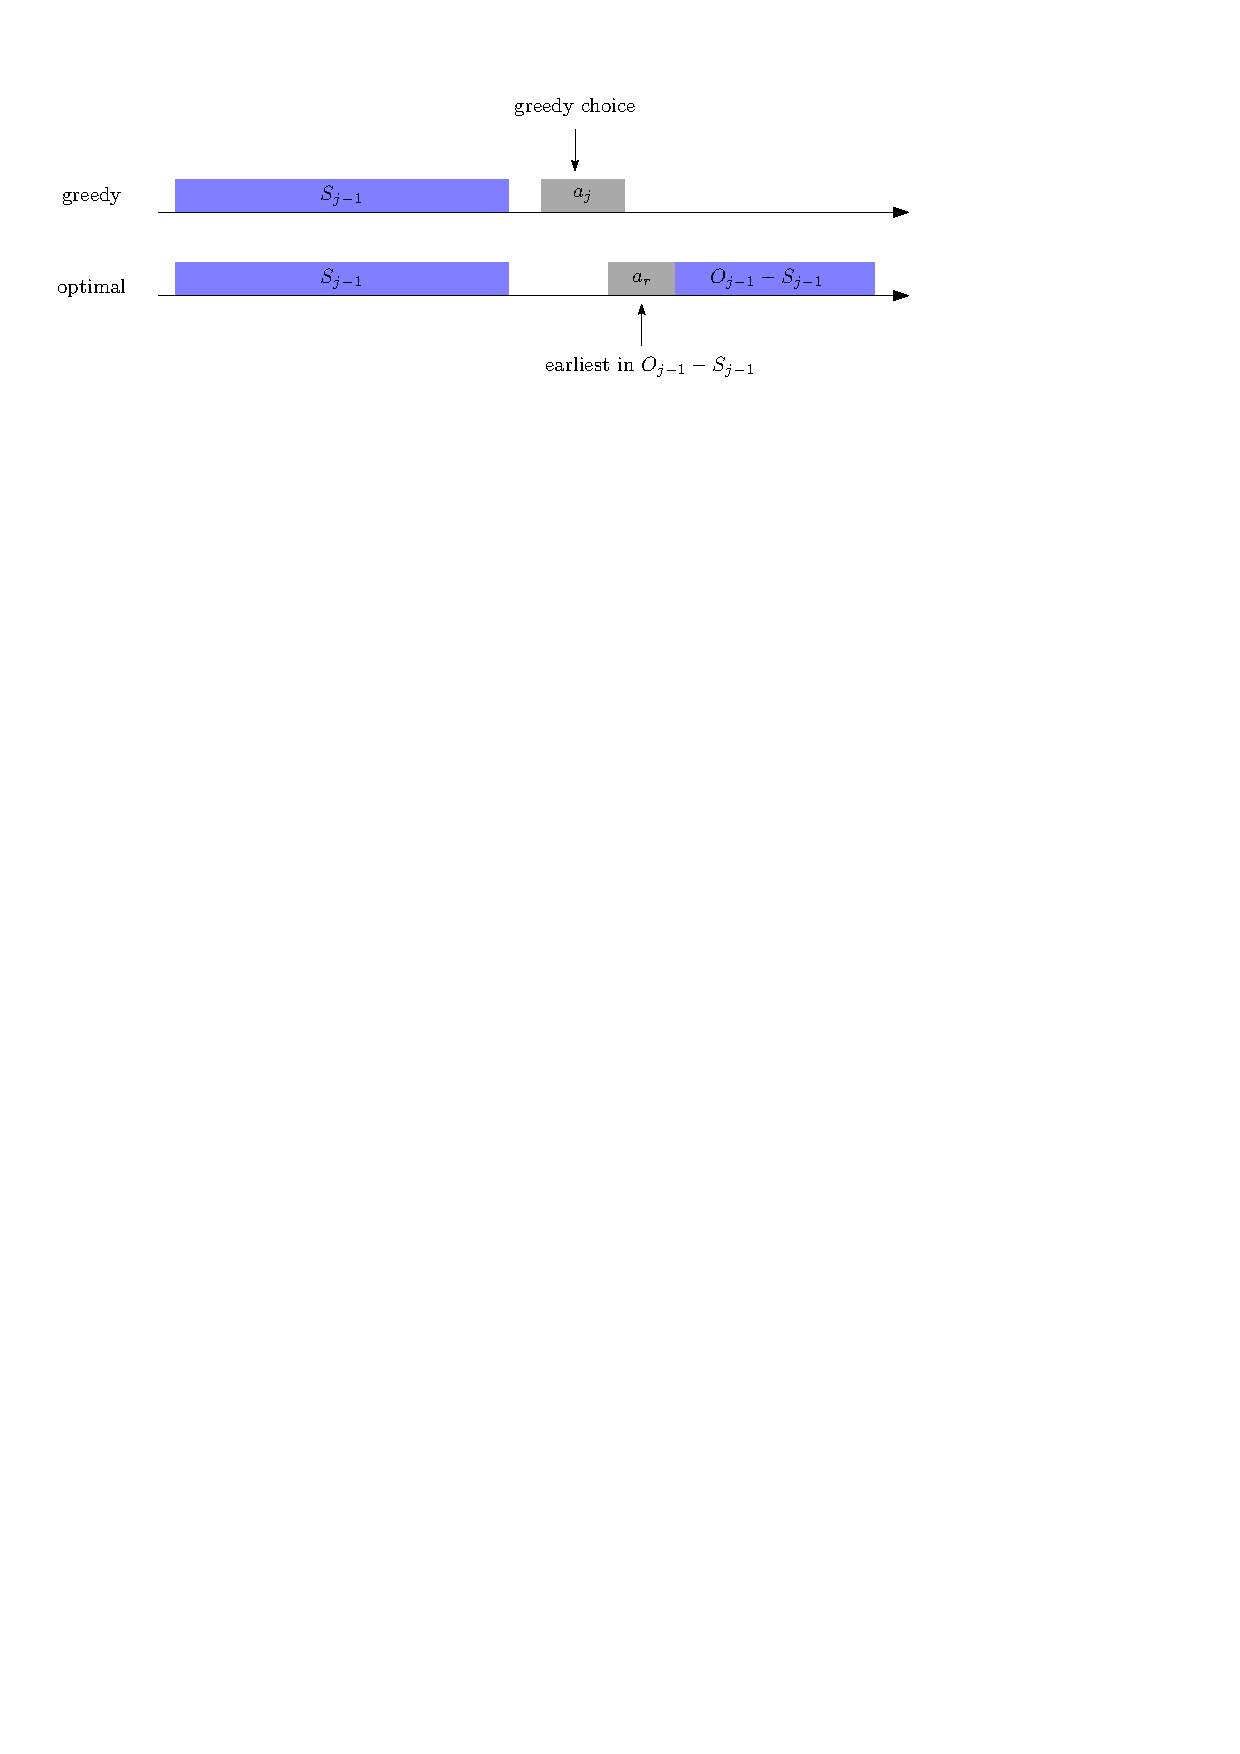
\includegraphics[width=0.7\linewidth]{greedy/interval-scheduling-optimality-proof.pdf}
    \end{center}
    By induction, the claim is true for all $k \in \{0,1,\ldots,n\}$.
\end{proof}

The previous two proofs use the technique known as the exchange argument. They both rely on the argument that if the greedy solution after $j$ iterations can be extended to an optimal solution, then the greedy solution after $j+1$ iterations can also be extended to an optimal solution by exchanging some interval with one chosen based on the greedy strategy. 

The last proof uses what we call an ``\textbf{charging argument}''. In this case, the charging argument charges each interval of an optimal solution (or arbitrary solution) to a unique interval in the greedy solution. Charging arguments are also used in approximation algorithms (for example, to prove that an algorithm is a $k$-approximation).

\begin{proof}[Proof (by charging argument)] \index{charging argument}
    Given a set of jobs $S = \{a_1,\ldots,a_n\}$, let $O$ be an optimal solution of the interval scheduling problem. Let $S'$ be the solution given by the greedy algorithm using earliest finish time. We want to find a one-to-one function $h:\, O \to S'$. For any job $j \in O$, define $h(j)$ as the interval $j' \in S'$ that intersects $j$ and has the earliest finish time amongst intervals in $S'$ intersecting $j$.

    We claim that the $h$ is well-defined so $h(j)$ must exists for all $j$. This is proved by contradiction. Suppose, for contradiction, that there exists a $j \in O$ where $h(j)$ as we defined does not exist. By definition, this means no interval in $S'$ intersects with $j$. This implies that $j$ is compatible with every interval in $S'$, so the greedy strategy would have selected $j$ and $j$ would be part of $S'$. But then if $j \in S'$, $j$ intersects with itself. This is a contradiction. $h(j)$ \textbf{exists} for all $j \in O$. Furthermore, $h(j)$ is \textbf{unique} because all intervals in $S'$ are mutually disjoint, and every interval in $S'$ that intersects $j$ have distinct finish time.

    We then show that $h$ is \textbf{injective}, similarly by contradiction. Assume that there are two intervals $j_1,j_2 \in O$ such that $h(j_1) = h(j_2) = j' \in S'$. Without loss of generality, suppose that the finish time of $j_1$ is earlier than $j_2$. $j_1$ and $j_2$ are disjoint because they are both in $O$, which implies that $f_1 \leq s_2 < f_2$. Since $j' \in S'$, the greedy algorithm must have encountered $j'$ before $j_1$ and $j_2$. Thus, $f' \leq f_1$. But then, this implies that $f' \leq f_1 \leq s_2 < f_2$. That is, $j'$ and $j_2$ do not overlap. This is a contradiction because if they do not intersect, $h(j_2) \neq j'$. Therefore, $h$ is injective.
    
    Since there exists an one-to-one function $h:\; O \to S'$, by the charging argument, the greedy algorithm for the interval scheduling problem is optimal.
\end{proof}

More generally, we have shown that $|O| \leq |S'|$, which implies the optimality of the algorithm (that the algorithm returns the maximum-size subset).

\section{Interval Coloring (Interval Partition)}

Let us know consider a modified version of the original interval scheduling problem. Suppose that we are given a set of intervals. We want to color all intervals so that intervals with the same color do not intersect while using the minimum number of colors. This problem is also known as the interval partitioning problem.

Similar to interval scheduling, let's take a look at the few possible choices for our greedy strategy:
\begin{itemize}
    \item Earliest start time
    \item Earliest finish time
    \item Shortest interval
    \item Fewest conflicts
\end{itemize}
We can show using counterexamples that the last three heuristics, earliest finish time, shortest interval, and fewest conflicts, do not work. We will prove that the earliest start time greedy choice gives us a globally optimal solution for the interval partitioning problem.

The proof for this is somewhat similar to the charging argument that we used to prove the optimality of interval scheduling. We attempt to bound the size of the solution set in order to show that it is optimal (miminal). In the charging argument, we bound the size by showing that there exists an one-to-one function. In this proof, we will skip that part and instead bound the size directly.

\begin{lemma} \label{lem:interval-partition-upper-bound}
    Given a set of intervals, let $d$ be the maximum number of intersecting intervals at any time. The number of partitions (colors) given by any algorithms that solve the interval partitioning problem must be at least $d$.
\end{lemma}

\begin{proof}
    By contradiction.
\end{proof}

\begin{lemma} \label{lem:interval-partition-lower-bound}
    Let $d$ be defined as in the previous lemma. The greedy algorithm using earliest start time produces a solution with at most $d$ partitions.
\end{lemma}

\begin{proof}
    Let $d'$ be the number of partitions produced by the greedy algorithm. Suppose for contradiction that the algorithm used more than $d$ partitions. Consider the first time that the greedy algorithm used $d+1$ partitions. Suppose this happens when the algorithm is trying to assign a partition to the interval $j$. This implies that there are $d$ intervals intersecting $j$. Let $s_j$ be the starting time of $j$. These $d$ intervals must contain $s_j$. This is because all the previous $d$ intervals have starting time earlier than $s_j$. So it must be that case that $s_j$ is after or at the starting time of the other $d$ intervals. But then, this implies that there are $d+1$ overlapping intervals at $s_j$, contradicting the fact that there are at most $d$ intersecting intervals at any time.
\end{proof}

\begin{corollary}
    The greedy algorithm produces a solution with exactly $d$ partitions.
\end{corollary}

\begin{proof}
    Follows immediately from the Lemma \ref{lem:interval-partition-upper-bound} and \ref{lem:interval-partition-lower-bound}.
\end{proof}

Hence the theorem:

\begin{theorem}
    The greedy algorithm using earliest starting time as greedy choice is optimal.
\end{theorem}

This greedy algorithm is implemented as follows. Suppose, as a precondition, that $S$ is sorted in increasing order of starting time, and that elements in $Q$ contains objects of $\proc{Interval}$s that are indexed by finish time.

\begin{codebox}
    \Procname{$\proc{Interval-Partitioning}(S)$}
    \li $d = 0$
    \zi \Comment{initialize PQ using finish time as key} 
    \li $Q = \proc{Priority-Queue}(\id{key}=f)$ 
    \li \For $i = 1$ \textbf{to} $\attrib{S}{length}$ \Do
        \li $k = \proc{Extract-Min}(Q)$
        \li \If $k \isequal \const{nil}$ \Then
            \li $d = d + 1$
            \li $\id{interval} = $ \textbf{new} $\proc{Interval}(i.f)$ 
            \li $\proc{Insert}(Q,\id{interval})$
        \End
        \li \If $i.s > \proc{Min}(Q)$ \Then
            \zi \Comment{if $i$ is compatible with $k$, allocate $i$ to $k$}
            \li $k.f = i.f$
            \li $\proc{Insert}(Q, k)$
        \li \Else
            \zi \Comment{otherwise, create new classroom $d+1$}
            \li $d = d + 1$
            \li $\proc{Insert}(Q, k)$
            \li $\id{interval} = $ \textbf{new} $\proc{Interval}(i.f)$
            \li $\proc{Insert}(Q,\id{interval})$
        \End
    \End
    \li \Return $d$
\end{codebox}

This algorithm runs in $O(n \log n)$ time. This is the case regardless of whether or not we consider sorting as part of the algorithm because the $n$ priority queue operation is going to cost $O(n \log n)$ anyway, assuming the priority is implemented as a min-heap.

\section{Greedy Strategy}

The greedy strategy can be generalized as follows:

\begin{enumerate}
    \item Cast the optimization problem as one in which we make a choice and are left with one subproblem to solve.
    \item Prove that there is always an optimal solution to the original problem that makes the greedy choice, so that the greedy choice is always safe.
    \item Demonstrate optimal substructure by showing (typically by contradiction or induction) that, having made the greedy choice, what remains is a subproblem with the property that if we combine an optimal solution to the subproblem with the greedy choice we have made, we arrive at an optimal solution to the original problem.
\end{enumerate}

\index{greedy property}
The important property that requires us to prove when implementing a greedy algorithm is the \textbf{greedy property}. It tells us that we can assemble a globally optimal solution from locally optimal choices. The exchange argument for the proof (the first two proofs that we have seen for interval scheduling) argues that we can modify the globally optimal solution to substitute the greedy choice for some other choice, resulting in one similar, but smaller, subproblem.

\chapter{Graph Algorithms}
\section{Interval Scheduling as Graph Problems}

\section{Minimum Spanning Tree}

\subsection{Kruskal's Algorithm}

\subsection{Prim's Algorithm}

\section{Single-Source Shortest Path}

\subsection{Dijkstra's Algorithm}

\chapter{Huffman Encoding}

\chapter{Generalizing and Formalizing Greedy Algorithms}
\section{Priority Model}

For a given problem, we assume that the input items belong to some set $\mathcal{J}$. For any execution of the algorithm, the input is a finite subset $\mathcal{I} \subset \mathcal{J}$.

Let $f:\,\mathcal{J} \to \R$ be a function. We do not place restriction on the complexity or computability of such function. For an input set $\mathcal{I} = \{I_1,\ldots,I_n\}$, the function induces a total ordering $\preceq$ on $\mathcal{I}$, breaking ties using certain rules (for example, by input ID).

For a fixed order priority algorithm, $f$ and $\preceq$ are set initially before the algorithm observes the input set. For adaptive order, the algorithm computes $f$ and $\preceq$ dynamically. More formally, there is a different function $f_i$ and ordering $\preceq_i$ associated with each iteration $i$ where $f_i$ and $\preceq$ depends on the items $\{I_1,\ldots,I_{j}\}$ considered in prior iterations $j < i$. 

Let us first consider fixed order algorithm under this priority model. In each iteration $k$ for $1 \leq k \leq n$, the algorithm observes input element $I_k \in \mathcal{I}$ and based on this input and all previous inputs and decisions, the algorithm makes an irrevocable decision $D_k$ about this input item (this typically involves whether to include or discard the current item).

This model gives us the following template for fixed order priority algorithms

\begin{codebox}
    \li $\mathcal{J} =$ set of all possible inputs
    \li $\preceq\,\, = $ a total ordering on $\mathcal{J}$ (typically induced by a function $f$)
    \li $\mathcal{I} \subset \mathcal{J} = $ actual input to the algorithm
    \li $S = \emptyset$ \RComment{items already examined by the algorithm}
    \li $i = 0$
    \li \While $\mathcal{I} - S \neq \emptyset$ \Do
        \li $i = i + 1$
        \li $\mathcal{I} = \mathcal{I} - S$
        \li $I_i = \min_{\preceq} \{ I \in \mathcal{I} \}$ \RComment{select min element based on the ordering $\preceq$}
        \li make an irrevocable decision $D_i$ concerning $I_i$ 
        \li $S = S \cup \{I_i\}$
    \End      
\end{codebox}

This template can be modified to allow the algorithm to determine the total ordering dynamically based on the elements it has observed so far.

\begin{codebox}
    \li $\mathcal{J} =$ set of all possible inputs
    \li $\mathcal{I} \subset \mathcal{J} = $ actual input to the algorithm
    \li $S = \emptyset$ \RComment{items already examined by the algorithm}
    \li $i = 0$
    \li \While $\mathcal{I} - S \neq \emptyset$ \Do
        \li $i = i + 1$
        \li $\preceq_i\,\, = $ a total ordering on $\mathcal{J}$ (typically induced by a function $f_i$)
        \li $\mathcal{I} = \mathcal{I} - S$
        \li $I_i = \min_{\preceq_i} \{ I \in \mathcal{I} \}$ \RComment{select min element based on the ordering $\preceq_i$}
        \li make an irrevocable decision $D_i$ concerning $I_i$ 
        \li $S = S \cup \{I_i\}$
        \li $\mathcal{J} = \mathcal{J} - \{I \in \mathcal{I} \mid I \preceq_i I_i \}$
    \End      
\end{codebox}

For greedy algorithm, the algorithm does not have knowledge of the input other than the elements it has observed so far. Sometimes, we allow the algorithm to have some easily computed global information such as the size of the input. The input is said to be chosen by an adversary.

This generalization applies to a broader category of algorithms known as priority-based algorithms. Informally, greedy algorithms always assume that the current iteration could be the last one and the current item being considered might as well be the last item. Hence, an optimal decision is immediate when the algorithm finishes. A more general priority algorithm that are not necessarily greedy does not have such restriction

This formalization was first given by Allan Borodin \textit{et al.} in \textit{(Incremental) Priority Algorithms} (Thirteen Annual ACM-SIAM Symposium on Discrete Algorithms, January 2002) \cite{borodin-priority}.

\section{Global Optimality of Greedy Algorithms}

(From Allan Borodin's notes)

Most greedy algorithms are not opitmal. The method we use to show that a greedy algorithm is optimal (when it is) known as the exchange argument often proceeds as follws. At each stage $i$, we define our partial solution to be promising if it can be extended to an optimal solution by using elements that haven't been considered yet by the algorithm; that is, a partial solution is promising after stage $i$ if there exists an optimal solution that is consistent with all the decisions made through stage $i$ by our partial solution. We prove the algorithm is optimal by fixing the input problem, and proving by induction on $i \geq 0$ that after stage $i$ is performed, the partial solution obtained is promising. The base case of $i=0$ is usually completely trivial: the partial solution after stage O is what we start with, which is usually the empty partial solution, which of course can be extended to an optimal solution. The hard part is always the induction step, which we prove as follmvs. Say that stage $i+1$ occurs, and that the partial solution after stage $i$ is $S_i$ and that the partial solution after stage $i+1$ is $S_{i+1}$, and we know that there is an optimal solution $S_{opt}$ that extends $S_i$; we want to prove that there is an optimal solution $S_{opt}'$ that extends $S_{i+1}$. $S_{i+1}$ extends $S_i$ by taking only one decision; if $S_{opt}$ makes the same decision, then it also extends $S_{i+1}$, and wve can just let $S_{opt}' = S_{op}$ and we are done. The hard part of the induction step is if $S_{opt}$ does not extend $S_{i+1}$, In this case, we have to show either that $S_{opt}$ could not have been optimal (implying that this case cannot happen), or we show how to change some parts of $S_{opt}$ to create a solution $S_{opt}'$ such that

\begin{itemize}
    \item $S_{opt}'$ extends $S_{i+1}$ and
    \item $S_{opt}'$ has value (cost, profit, etc.) at least as good as $S_{opt}$, so the fact that $S_{opt}$ is optimal implies that $S_{opt}'$ is optimal.
\end{itemize}

For most greedy algorithms, when it ends, it has constructed a solution that cannot be extended to any solution other than itself. Therefore, if we have proven the above, we know that the solution constructed by the greedy algorithm must be optimal.

\part{Dynamic Programming}

\chapter{Introduction to Dynamic Programming}
\section{Dynamic Programming} \index{dynamic programming} \index{memoization}

\textbf{Dynamic programming} is a method for solving complex problem by breaking it down to a collection of simpler subproblems, solving each of those subproblems, and storing their solutions. The next time the same subproblem occurs, instead of recomputing the solution, the algorithm can just use the previously computed solution. Each subproblem is indexed in some way to facilitate the lookup. The technique of storing solutions to subproblems is called \textbf{memoization}.

\part{Network Flow}

\part{Complexity}

\part{Linear Programming}

\part{Approximation Algorithms}

\part{Randomized Algorithms}

%----------------------------------------------------------------------------------------
%	APPENDIX
%----------------------------------------------------------------------------------------
\part*{Appendix}
\appendix
\chapter*{Commonly Used Axioms \& Theorems}
\addcontentsline{toc}{chapter}{\textcolor{ocre}{Axioms \& Theorems}} 

\renewcommand{\leftmark}{\sffamily\bfseries Axioms \& Theorems}
\renewcommand{\rightmark}{\sffamily\bfseries Axioms \& Theorems}

\section*{Rules of Inference} \label{rulesofinference}

\begin{axiom_appendix}[Modus Ponens]
$(P \wedge (P \implies Q)) \implies Q $
\end{axiom_appendix}

\begin{axiom_appendix}[Modus Tollens]
$(\neg Q \wedge (P \implies Q)) \implies \neg P $
\end{axiom_appendix}

\begin{axiom_appendix}[Hypothetical Syllogism (transitivity)]
\hfill

$((P \implies Q) \wedge (Q \implies R)) \implies (P \implies R) $
\end{axiom_appendix}

\begin{axiom_appendix}[Disjunctive Syllogism]
$((P \vee Q) \wedge \neg P) \implies Q$
\end{axiom_appendix}

\begin{axiom_appendix}[Addition]
$P \implies (P \vee Q)$
\end{axiom_appendix}

\begin{axiom_appendix}[Simplification]
$(P \wedge Q) \implies P$
\end{axiom_appendix}

\begin{axiom_appendix}[Conjunction]
$((P) \wedge (Q)) \implies (P \wedge Q)$
\end{axiom_appendix}

\begin{axiom_appendix}[Resolution]
$((P \vee Q) \wedge (\neg P \vee R)) \implies (Q \vee R)$
\end{axiom_appendix}

\section*{Laws of Logic}

\begin{axiom_appendix}[Implication Law]
$(P \implies Q) \equiv (\neg P \vee Q)$
\end{axiom_appendix}

\begin{axiom_appendix}[Distributive Law]
\begin{align*}
    (P \wedge (Q \vee R)) &\equiv ((P \wedge Q) \vee (P \wedge R)) \\
    (P \vee (Q \wedge R)) &\equiv ((P \vee Q) \wedge (P \vee R))
\end{align*}
\end{axiom_appendix}

\begin{axiom_appendix}[De Morgan's Law]
\begin{align*}
    \neg (P \wedge Q) &\equiv (\neg P \vee \neg Q) \\
    \neg (P \vee Q) &\equiv (\neg P \wedge \neg Q)
\end{align*}
\end{axiom_appendix}

\begin{axiom_appendix}[Absorption Law]
\begin{align*}
    (P \vee (P \wedge Q)) &\equiv P \\
    (P \wedge (P \vee Q)) &\equiv P
\end{align*}
\end{axiom_appendix}

\begin{axiom_appendix}[Commutativity of AND]
$A \wedge B \equiv B \wedge A$
\end{axiom_appendix}

\begin{axiom_appendix}[Associativity of AND]
$(A \wedge B) \wedge C \equiv A \wedge (B \wedge C)$
\end{axiom_appendix}

\begin{axiom_appendix}[Identity of AND]
$\textbf{T} \wedge A \equiv A$
\end{axiom_appendix}

\begin{axiom_appendix}[Zero of AND]
$\textbf{F} \wedge A \equiv \textbf{F}$
\end{axiom_appendix}

\begin{axiom_appendix}[Idempotence for AND]
$A \wedge A \equiv A$
\end{axiom_appendix}

\begin{axiom_appendix}[Contradiction for AND]
$A \wedge \neg A \equiv \textbf{F}$
\end{axiom_appendix}

\begin{axiom_appendix}[Double Negation]
$\neg (\neg A) \equiv A$
\end{axiom_appendix}

\begin{axiom_appendix}[Validity for OR]
$A \vee \neg A \equiv \textbf{T}$
\end{axiom_appendix}

\section*{Induction}

\vspace{\parskip}

\begin{axiom_appendix}[Well Ordering Principle]
Every nonempty set of nonnegative integers has a smallest element. i.e., For any $A \subset \N$ such that $A \neq \emptyset$, there is some $a \in A$ such that $\forall a' \in A.a\leq a'$.
\end{axiom_appendix}

\section*{Recurrences}

\vspace{\parskip}

\begin{theorem_appendix}[The Master Theorem]
Suppose that for $n \in \Z^+$.
\begin{equation*}
    T(n) =
    \begin{cases}
    c & \text{if $n<B$} \\
    a_1 T(\lceil n/b \rceil) + a_2 T(\lfloor n/b \rfloor) + dn^i & \text{if $n\geq B$}
    \end{cases}
\end{equation*}
where $a_1, a_2, B, b \in \N$.

Let $a = a_1+a_2 \geq 1$, $b>1$, and $c,d,i \in \R \cup \{0\}$. Then,
\begin{equation*}
    T(n) \in
    \begin{cases}
    O(n^i \log n) & \text{if $a=b^i$} \\
    O(n^i) & \text{if $a < b^i$} \\
    O(n^{\log_b a}) & \text{if $a > b^i$}
    \end{cases}
\end{equation*}
\end{theorem_appendix}

Linear Recurrences:

A linear recurrence is an equation
$$
f(n) = \underbrace{a_1 f(n-1) + a_2 f(n-2) + \cdots + a_d f(n-d)}_{\text{homogeneous part}}  + \underbrace{g(n)}_{\text{inhomogeneous part}}
$$
along with some boundary conditions.

The procedure for solving linear recurrences are as follows:

\begin{enumerate}
    \item Find the roots of the characteristic equation. Linear recurrences usually have exponential solutions (such as $x^n$). Such solution is called the \textbf{homogeneous solution}.
    $$
    x^n = a_1 x^{n-1} + a_2 x^{n-2} + \cdots + a_{k-1} x + a_k
    $$
    \item Write down the homogeneous solution. Each root generates one term and the homogeneous solution is their sum. A non-repeated root $r$ generates the term $cr^n$, where $c$ is a constant to be determined later. A root with $r$ with multiplicity $k$ generates the terms
    $$
    d_1r^n \quad d_2nr^n \quad d_3n^2r^n \quad \cdots \quad d_kn^{k-1}r^n
    $$
    where $d_1,\cdots,d_k$ are constants to be determined later.
    \item Find a \textbf{particular solution} for the full recurrence including the inhomogeneous part, but without considering the boundary conditions.
    
    If $g(n)$ is a constant or a polynomial, try a polynomial of the same degree, then of one higher degree, then two higher. If $g(n)$ is exponential in the form $g(n) = k^n$, then try $f(n) = ck^n$, then $f(n) = (bn+c)k^n$, then $f(n) = (an^2+bn+c)k^n$, etc.
    
    \item Write the \textbf{general solution}, which is the sum of homogeneous solution and particular solution.
    \item Substitute the boundary condition into the general solution. Each boundary condition gives a linear equation. Solve such system of linear equations for the values of the constants to make the solution consistent with the boundary conditions.
\end{enumerate}


\chapter*{Basic Prerequisite Mathematics}
\addcontentsline{toc}{chapter}{\textcolor{ocre}{Basic Prerequisite Mathematics}}
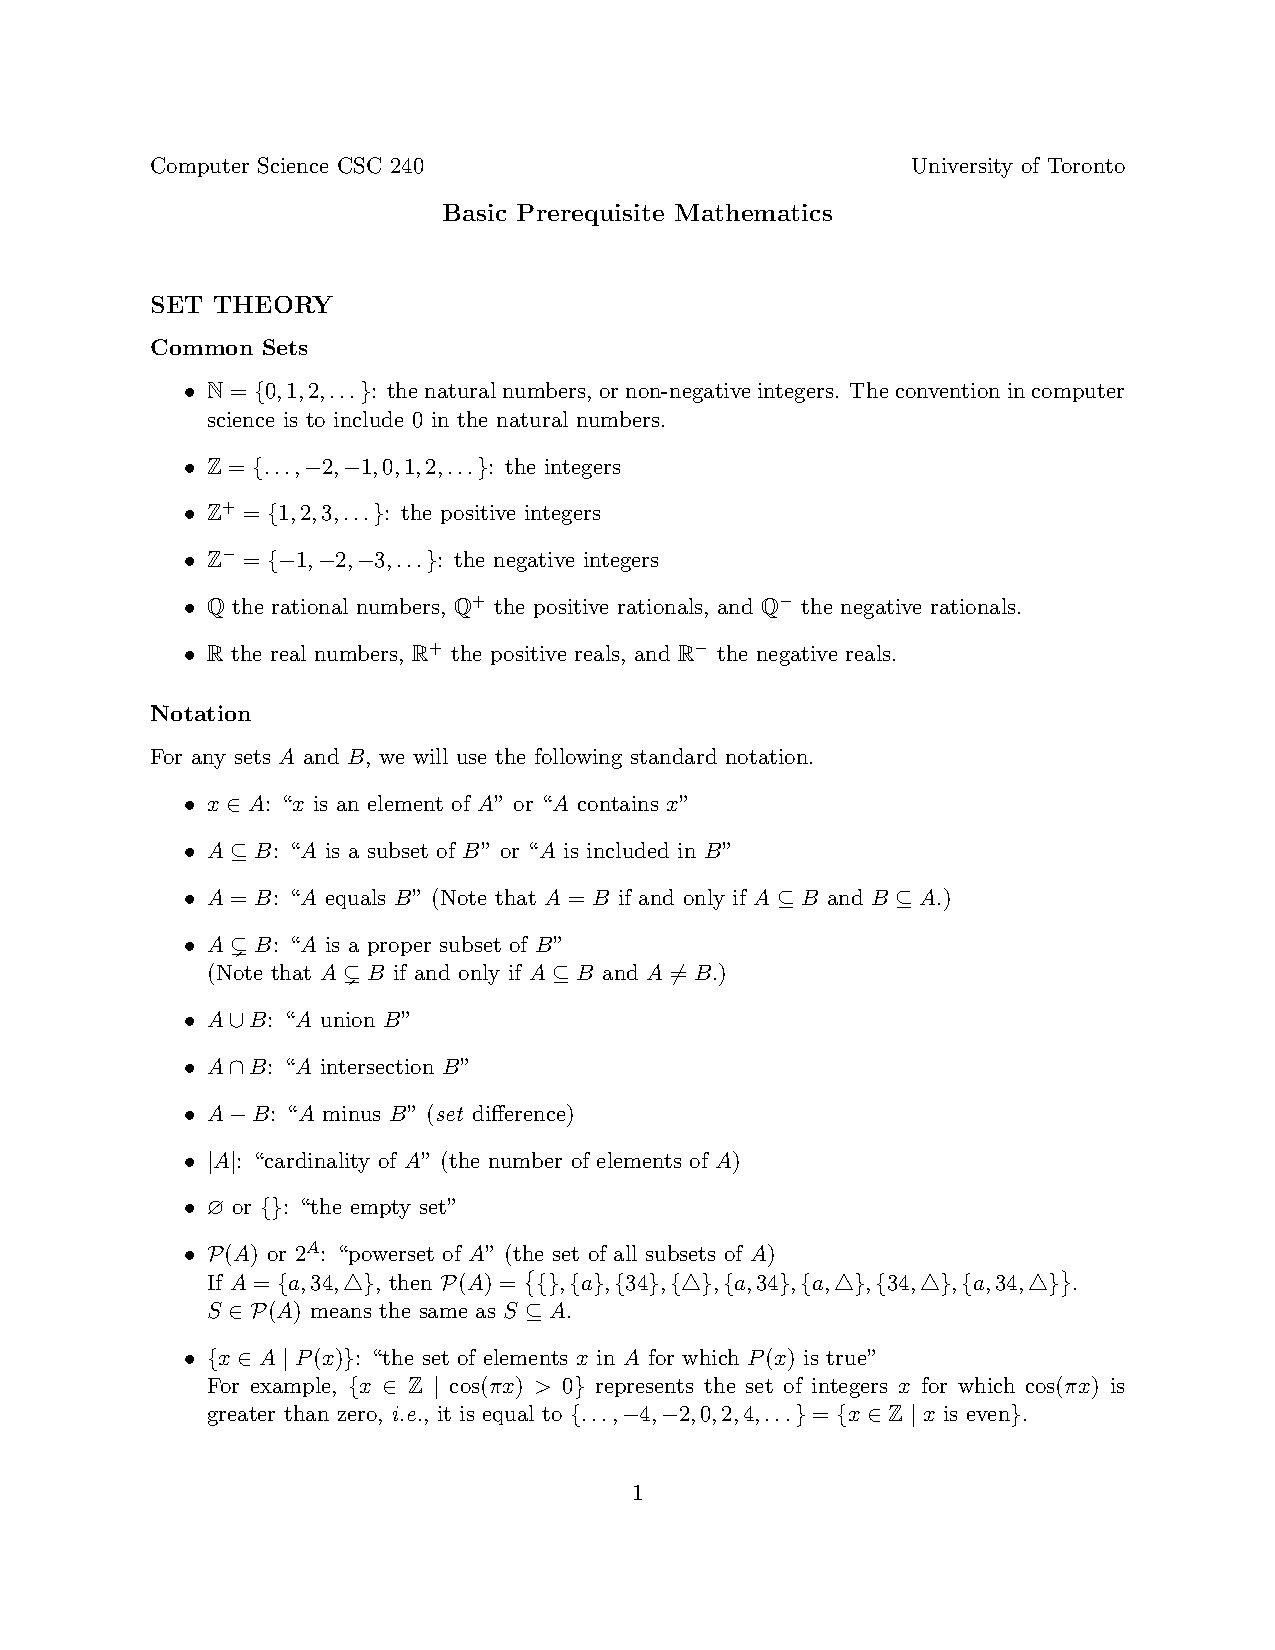
\includepdf[pages=-]{appendix/basicMath.pdf}

\chapter*{Proof Templates}
\addcontentsline{toc}{chapter}{\textcolor{ocre}{Proof Templates}}
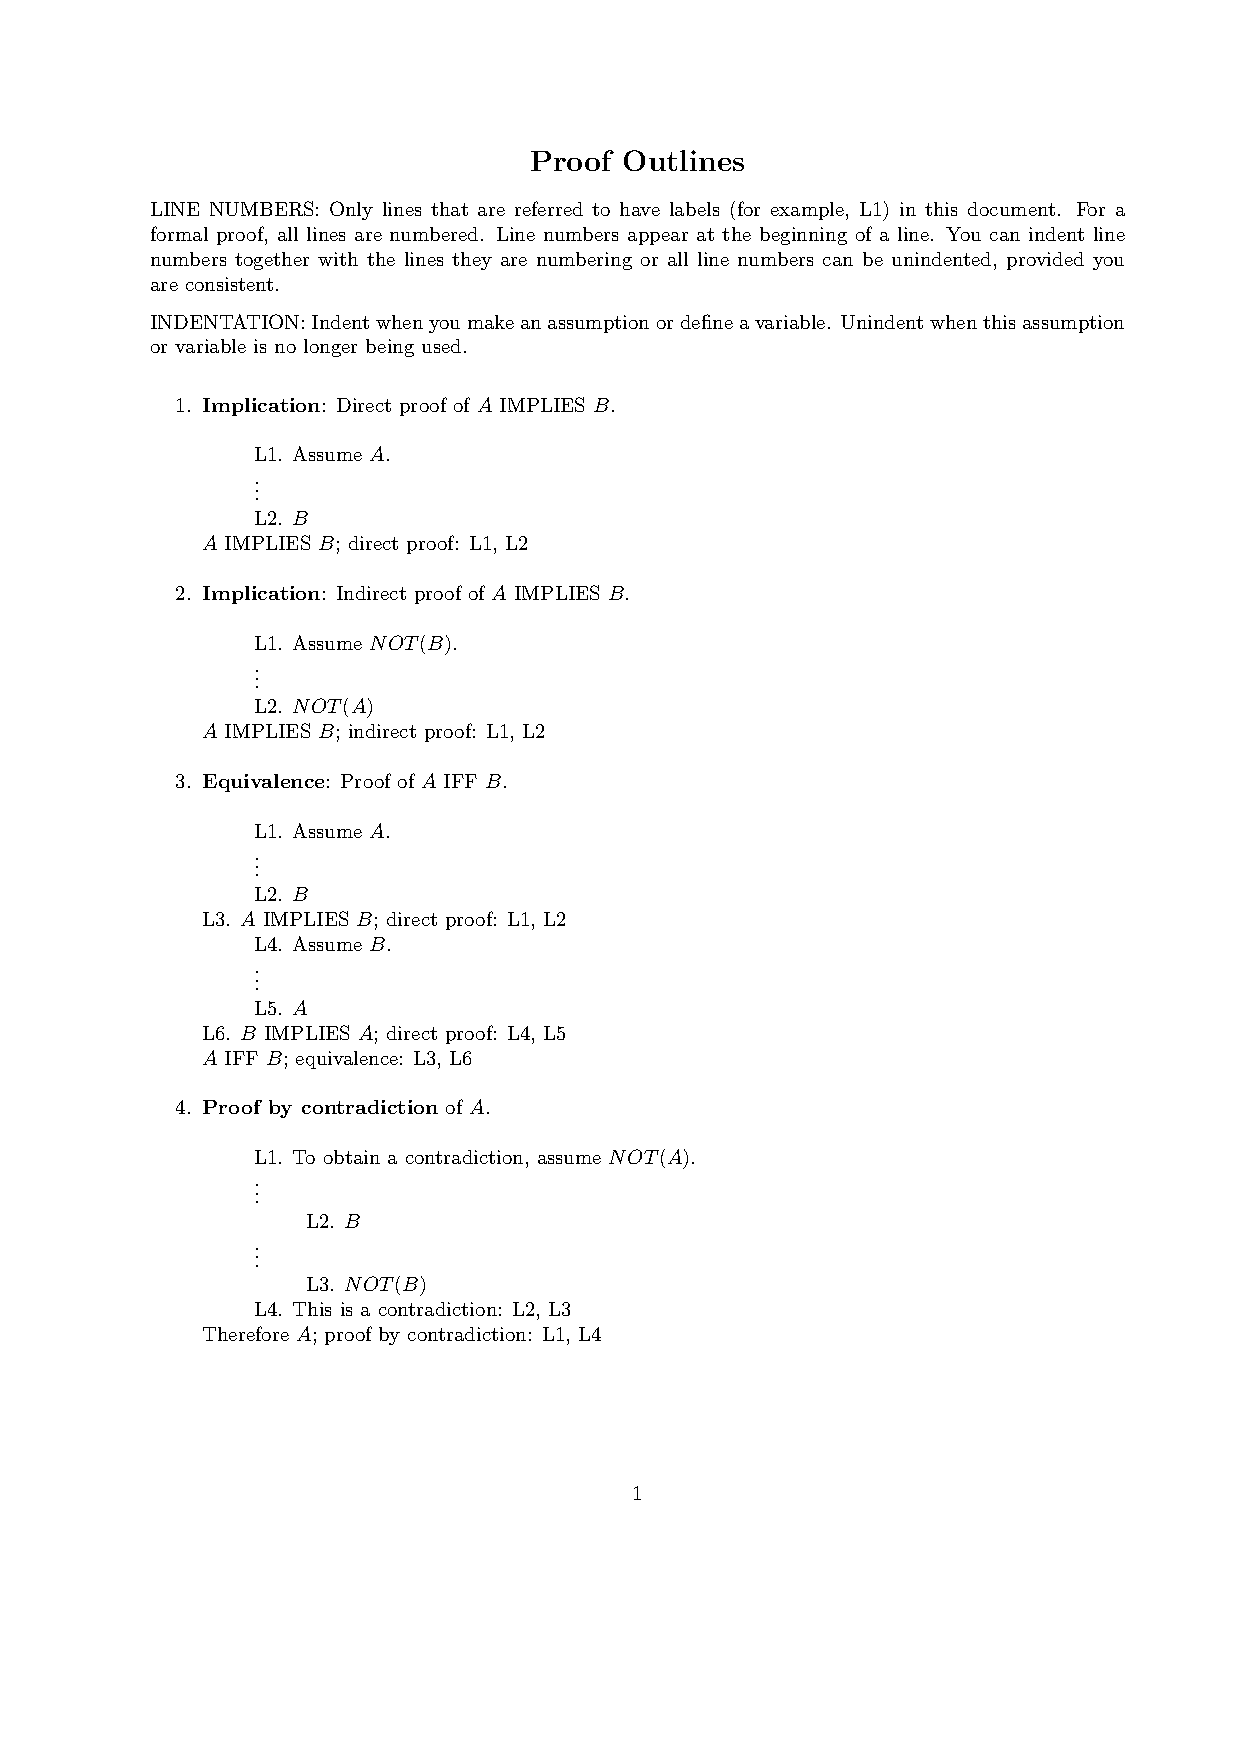
\includepdf[pages=-]{appendix/proofOutlines.pdf}

%----------------------------------------------------------------------------------------
%	INDEX
%----------------------------------------------------------------------------------------

\chapter*{Index}
\renewcommand{\leftmark}{\sffamily\bfseries Index}
\renewcommand{\rightmark}{\sffamily\bfseries Index}
%\cleardoublepage % Make sure the index starts on an odd (right side) page
\setlength{\columnsep}{0.75cm} % Space between the 2 columns of the index
\addcontentsline{toc}{chapter}{\textcolor{ocre}{Index}} % Add an Index heading to the table of contents

\printindex % Output the index

%------------------------------------------------
%   BIBLIOGRAPHY ENTRIES
%------------------------------------------------
\chapter*{Bibliography}
\renewcommand{\leftmark}{\sffamily\bfseries Bibliography}
\renewcommand{\rightmark}{\sffamily\bfseries Bibliography}
\addcontentsline{toc}{chapter}{\textcolor{ocre}{Bibliography}} % Add a Bibliography heading to the table of contents

\section*{Courses}
\addcontentsline{toc}{section}{Courses}
\printbibliography[heading=bibempty,type=misc]

\section*{Books}
\addcontentsline{toc}{section}{Books}
\printbibliography[heading=bibempty,type=book]

\section*{Journal Articles}
\addcontentsline{toc}{section}{Journal Articles}
%\printbibliography[heading=bibempty,type=article]

\newpage

%------------------------------------------------
%   TUTORIALS
%------------------------------------------------

%----------------------------------------------------------------------------------------

\end{document}
